\documentclass[10pt,openany]{book}
\usepackage{iftex}
\ifPDFTeX
\usepackage[utf8]{inputenc}
\DeclareUnicodeCharacter{2212}{\ensuremath{-}}
\DeclareUnicodeCharacter{2192}{\ensuremath{\to}}
\DeclareUnicodeCharacter{03B1}{\ensuremath{\alpha}}
\fi
\usepackage[T1]{fontenc}
\usepackage{lmodern}
\AtBeginDocument{\normalfont\DeclareFontShape{T1}{lmr}{bx}{sc}{<->ssub*lmr/m/sc}{}}
\usepackage[spanish,es-nodecimaldot]{babel}
\spanishplainpercent
\AtBeginDocument{\spanishdeactivate{"~<>}}
\usepackage[a4paper,margin=2.5cm,headheight=14pt]{geometry}
\usepackage{needspace}
\usepackage{amsmath,amssymb,mathtools,booktabs,array,longtable,graphicx,xcolor,tikz,enumitem,microtype,titlesec,fancyhdr}
\usepackage[breakable,skins]{tcolorbox}
\usepackage[labelfont=bf]{caption}
\usepackage[hyphens]{url}
\usepackage[hidelinks,unicode,hypertexnames=false]{hyperref}
\definecolor{studiumInk}{RGB}{20,44,64}
\definecolor{studiumBlue}{RGB}{24,74,130}
\definecolor{studiumCyan}{RGB}{0,184,205}
\definecolor{studiumLight}{RGB}{232,240,250}
\definecolor{studiumWorkedBack}{RGB}{255,244,230}
\definecolor{studiumWorkedFrame}{RGB}{138,78,12}
\definecolor{studiumCheckBack}{RGB}{243,236,248}
\definecolor{studiumCheckFrame}{RGB}{96,48,130}
\titleformat{\chapter}[display]{\normalfont\filright}{\large\mdseries\scshape\chaptertitlename\ \thechapter}{1ex}{\normalfont\huge\bfseries}
\titlespacing*{\chapter}{0pt}{2.5ex plus 1ex minus .2ex}{2.3ex}
\titleformat{name=\chapter,numberless}[display]{\normalfont\filright}{}{0pt}{\normalfont\huge\bfseries}
\titleformat{\section}{\Large\bfseries}{\thesection}{.8em}{}
\titleformat{\subsection}{\large\bfseries}{\thesubsection}{.7em}{}
\makeatletter
\renewcommand*\l@section{\@dottedtocline{1}{1.5em}{3.5em}}
\makeatother
\setcounter{secnumdepth}{2}\setcounter{tocdepth}{2}
\setlength{\parindent}{1.5em}\setlength{\parskip}{3pt plus .5pt}
\setlength{\emergencystretch}{1.5em}\raggedbottom
\setlist{itemsep=2pt,topsep=4pt,leftmargin=*}
\setlist[description]{style=nextline,leftmargin=0pt,labelwidth=0pt,labelindent=0pt}
\allowdisplaybreaks[2]
\graphicspath{{figures/}}
\newcommand{\Raire}{287.05287}
\newcommand{\gzero}{9.80665}
\tcbset{studiumcommon/.style={breakable,boxrule=.65pt,arc=.7pt,left=1.7mm,right=1.7mm,top=1.3mm,bottom=1.3mm,before skip=10pt,after skip=10pt,fonttitle=\bfseries}}
\newtcolorbox{studiumworked}[1]{studiumcommon,colback=studiumWorkedBack,colframe=studiumWorkedFrame,colbacktitle=studiumWorkedFrame,coltitle=white,title={#1}}
\newcommand{\objetivos}[1]{\par\noindent\textbf{Objetivos de aprendizaje.} \textit{#1}\par\medskip}
\newcommand{\caja}[2]{\begin{tcolorbox}[studiumcommon,colback=studiumLight,colframe=studiumBlue,colbacktitle=studiumBlue,coltitle=white,title={#1}]#2\end{tcolorbox}}
\newcommand{\resumen}[1]{\begin{tcolorbox}[studiumcommon,colback=studiumCheckBack,colframe=studiumCheckFrame,colbacktitle=studiumCheckFrame,coltitle=white,title=Resumen]#1\end{tcolorbox}}
\newcommand{\figura}[2]{\begin{figure}[tbp]\centering\includegraphics[width=.83\linewidth]{#1.pdf}\caption{#2}\label{fig:#1}\end{figure}\noindent La figura~\ref{fig:#1} ofrece una representación del modelo discutido.}
\pagestyle{fancy}\fancyhf{}
\fancyhead[LE]{\small\thepage\hspace{1.5em}\mdseries\scshape\nouppercase{\leftmark}}
\fancyhead[RO]{\small\mdseries\scshape\nouppercase{\rightmark}\hspace{1.5em}\thepage}
\renewcommand{\headrulewidth}{.4pt}\renewcommand{\footrulewidth}{0pt}
\fancypagestyle{plain}{\fancyhf{}\fancyfoot[C]{\small\thepage}\renewcommand{\headrulewidth}{0pt}}

% Adaptación de la plantilla final de Motores Cohete. Fotografía GEnx: Olivier Cleynen, CC BY-SA 3.0.
\addto\captionsspanish{\renewcommand{\contentsname}{Índice}\renewcommand{\tablename}{Cuadro}\renewcommand{\listtablename}{Índice de cuadros}}
\numberwithin{equation}{chapter}
\let\cleardoublepage\clearpage
\fancyfoot[R]{\scriptsize\sffamily\color{studiumInk}En revisión}
\renewcommand{\chaptermark}[1]{\markboth{Capítulo \thechapter.\ #1}{}}
\renewcommand{\sectionmark}[1]{\markright{\thesection\ #1}}
\definecolor{studiumTipBack}{RGB}{232,244,236}
\definecolor{studiumTipFrame}{RGB}{27,107,58}
\newcommand{\consejo}[2]{\begin{tcolorbox}[studiumcommon,colback=studiumTipBack,colframe=studiumTipFrame,colbacktitle=studiumTipFrame,coltitle=white,title={#1}]#2\end{tcolorbox}}
\newcommand{\estado}{Edición íntegra de estudio. Pendiente de revisión experta independiente.}
\newcommand{\portada}[3]{%
\hypersetup{pageanchor=false}
\begin{titlepage}\thispagestyle{empty}
\begin{tikzpicture}[remember picture,overlay,x=1bp,y=-1bp]
\begin{scope}[shift={(current page.north west)}]
\clip (0,0) rectangle (595.276,841.89);
\fill[white] (0,0) rectangle (595.276,841.89);
% Fotografía original conservada; encuadre proporcional en la ventana de portada.
\IfFileExists{figures/portada.jpg}{%
 \begin{scope}
 \clip (0,89.5) rectangle (595.276,585.5);
 \node[inner sep=0pt] at (297.638,337.5){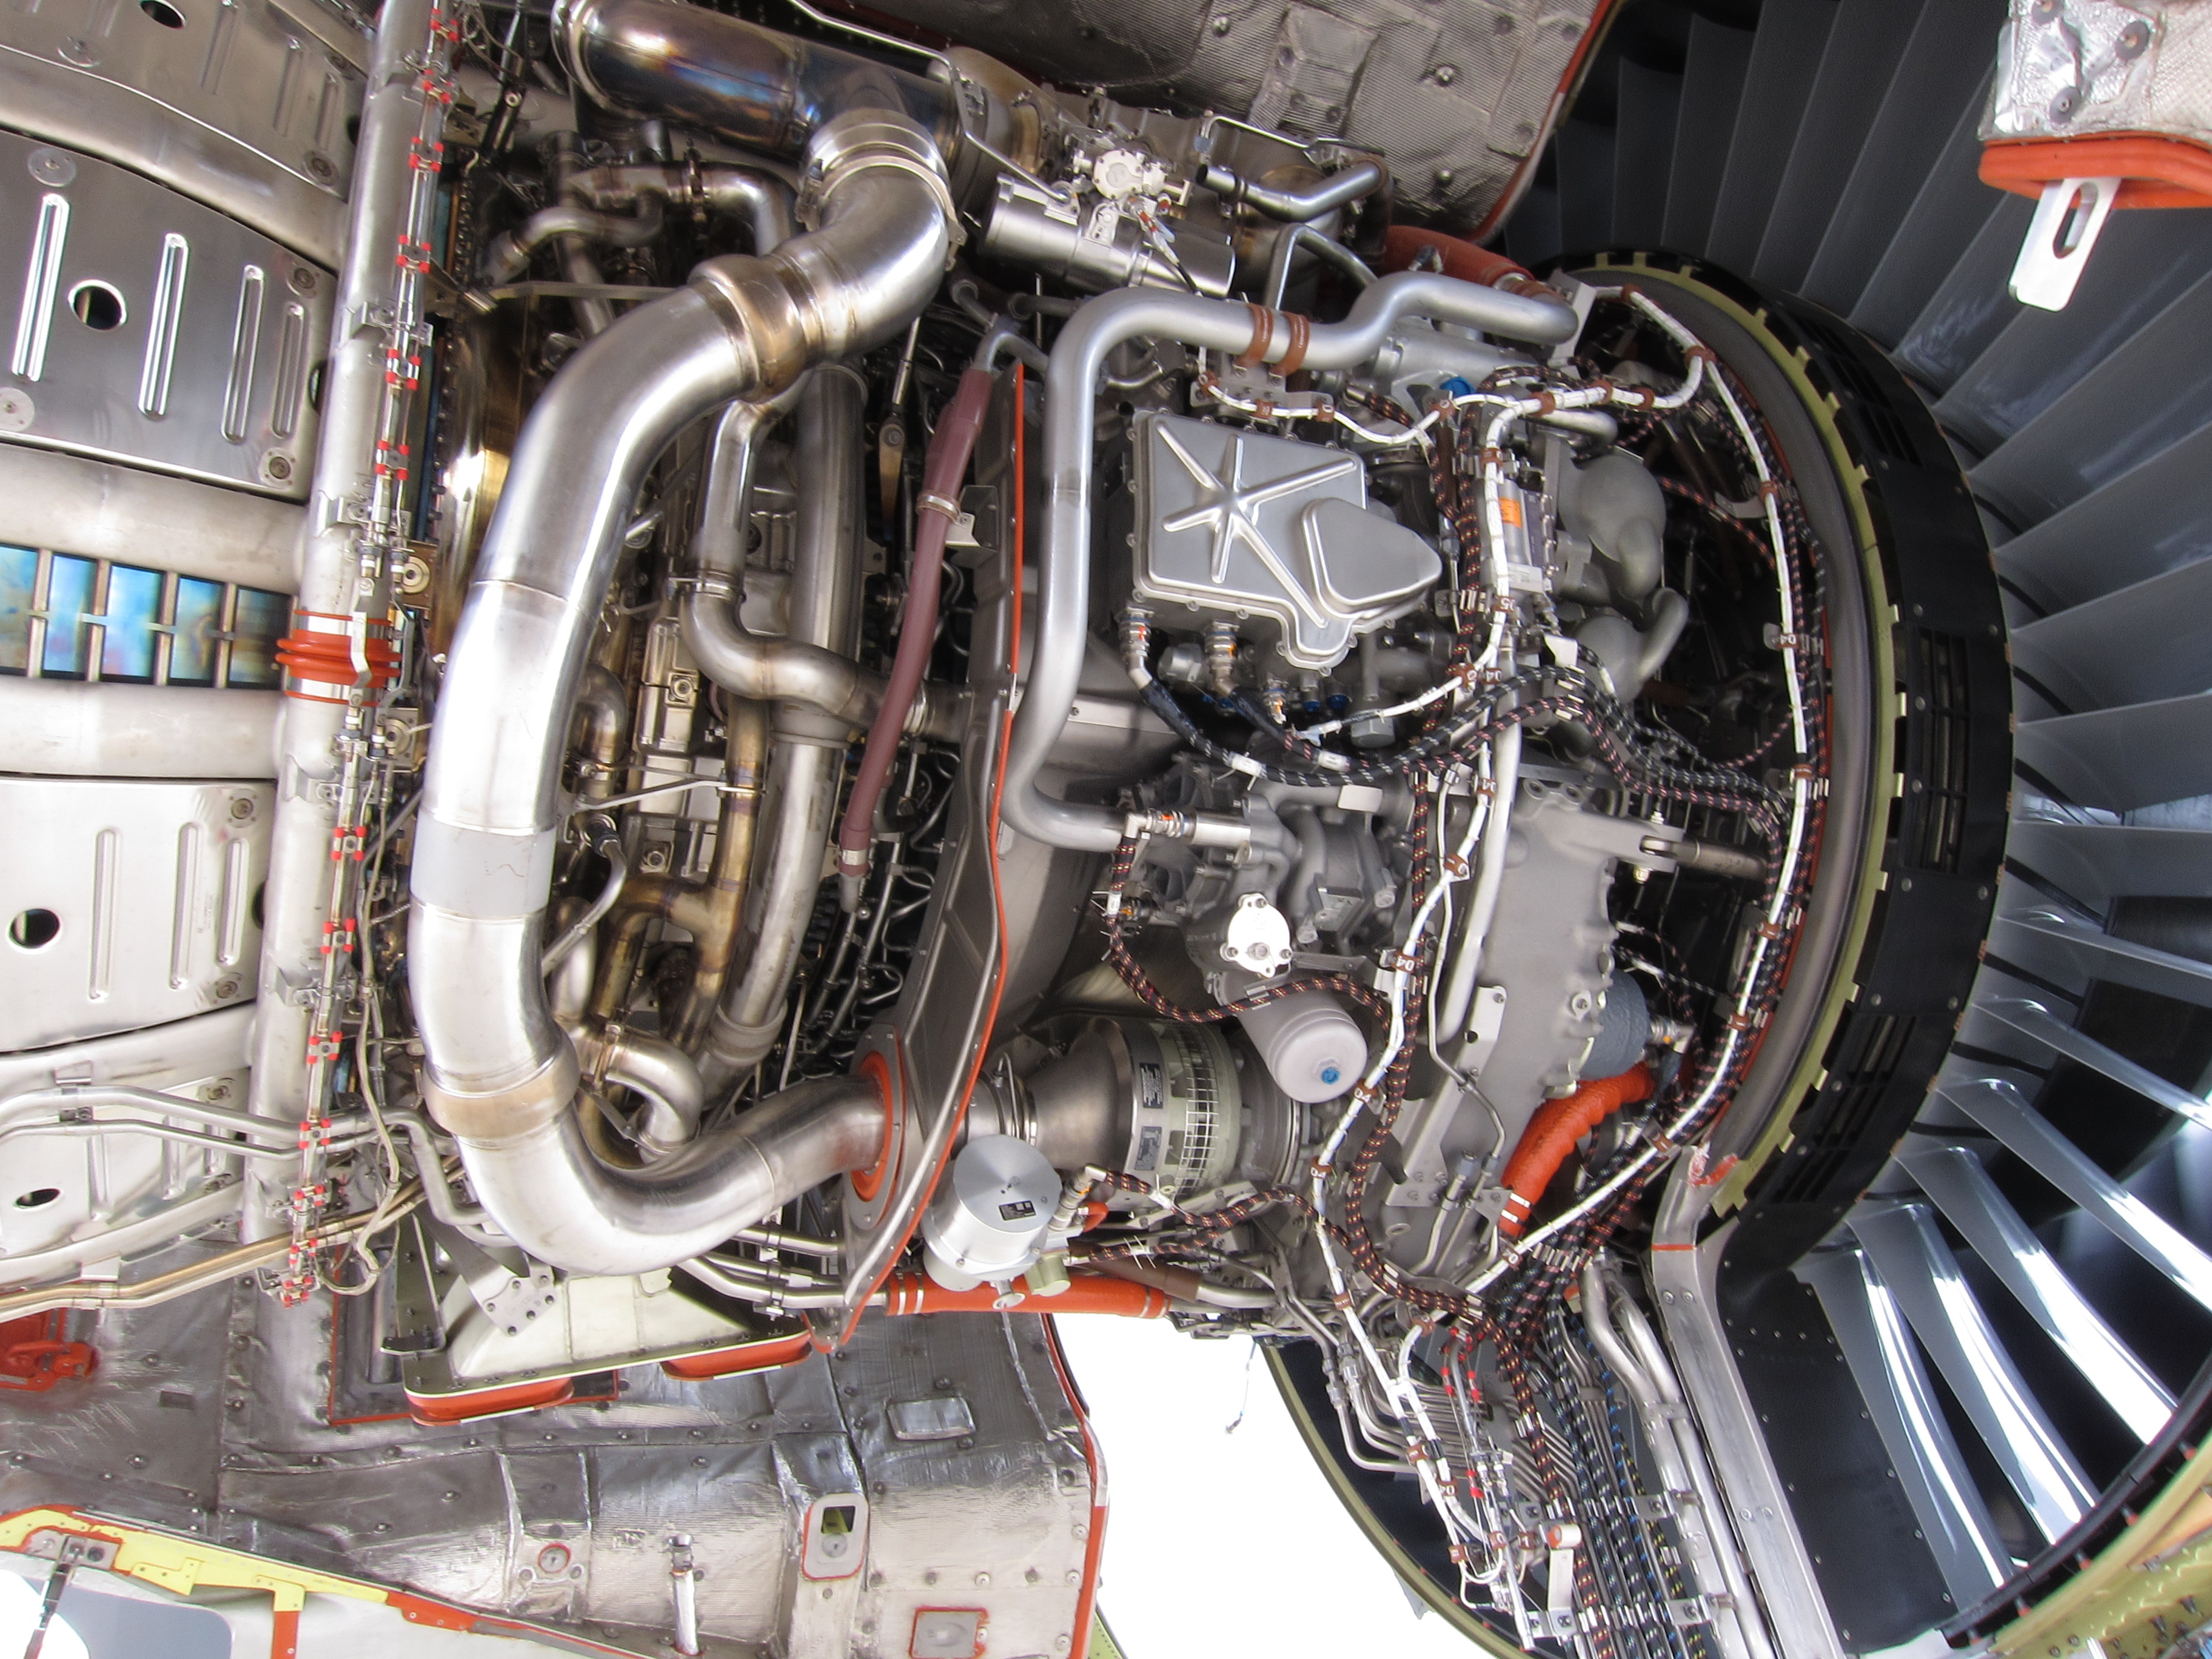
\includegraphics[height=496bp]{portada.jpg}};
 \end{scope}
}{%
 \fill[studiumLight!40!white] (0,89.5) rectangle (595.276,585.5);
 \node[text=studiumInk!45,font=\sffamily\fontsize{10}{13}\selectfont,align=center]
 at (297.638,535){Fotografía definitiva pendiente};
}
\fill[white,opacity=.91] (0,0) rectangle (595.276,89.5);
\fill[studiumInk,opacity=.96] (0,585.5) rectangle (595.276,841.89);
\node[anchor=west,text=studiumInk,font=\sffamily\bfseries\fontsize{18}{20}\selectfont,inner sep=0pt] at (51.223,38.5){STUDIUM};
\node[anchor=east,text=studiumInk,font=\sffamily\fontsize{8}{10}\selectfont,inner sep=0pt] at (544.05,38.5){EN REVISIÓN};
\fill[studiumCyan] (51.223,61.5) rectangle (80.8,63.7);
\node[anchor=west,text=studiumInk,font=\sffamily\fontsize{9}{11}\selectfont,inner sep=0pt] at (89.49,65.5){BIBLIOTECA DE INGENIERÍA};
\node[anchor=west,text=studiumCyan,font=\sffamily\bfseries\fontsize{10}{12}\selectfont,inner sep=0pt] at (51.223,608){#1};
\node[anchor=north west,text=white,text width=493pt,font=\rmfamily\bfseries\fontsize{27}{30}\selectfont,inner sep=0pt] at (51.223,627){#2};
\node[anchor=north west,text=white!82!studiumInk,text width=493pt,font=\sffamily\fontsize{11}{14}\selectfont,inner sep=0pt] at (51.223,730){#3};
\node[anchor=west,text=white,font=\sffamily\bfseries\fontsize{10}{12}\selectfont,inner sep=0pt] at (51.223,774){GRADO EN INGENIERÍA AEROESPACIAL};
\node[anchor=west,text=white!82!studiumInk,font=\sffamily\fontsize{10}{12}\selectfont,inner sep=0pt] at (51.223,789){Universidad de León};
\draw[white!75!studiumInk,line width=.4pt] (51.223,801) -- (544.05,801);
\node[anchor=west,text=white!82!studiumInk,font=\sffamily\fontsize{10}{12}\selectfont,inner sep=0pt] at (51.223,822){2026};
\node[anchor=east,text=white,font=\sffamily\bfseries\fontsize{10}{12}\selectfont,inner sep=0pt] at (544.05,822){Primera edición};
\end{scope}\end{tikzpicture}\null
\end{titlepage}\hypersetup{pageanchor=true}}

\newcommand{\creditosportada}{%
\par\noindent\begin{minipage}{\linewidth}\footnotesize
\textbf{Fotografía de portada.} Detalle del núcleo de un motor General Electric GEnx, Olivier Cleynen (21 de junio de 2011). Fuente: \href{https://commons.wikimedia.org/wiki/File:Detail_of_GEnx_turbofan_engine_core.jpg}{Wikimedia Commons}. Licencia: \href{https://creativecommons.org/licenses/by-sa/3.0/}{CC BY-SA 3.0}.
\par\noindent Se presenta con un recorte de encuadre y superposición de la composición editorial. La fotografía y su adaptación de encuadre mantienen la licencia CC BY-SA 3.0; no se atribuye al fotógrafo respaldo de esta edición.
\end{minipage}\par}

\newcommand{\caso}[2]{\begin{studiumworked}{#1}#2\end{studiumworked}}
\newcommand{\ilustra}[2]{\begin{figure}[htbp]\centering\includegraphics[width=.94\linewidth]{#1.pdf}\caption{#2}\label{fig:#1}\end{figure}}
\newcommand{\fuentes}[1]{\par\medskip\noindent{\footnotesize\textbf{Fuentes y localizadores.} #1}\par}
\newcommand{\apartado}[2]{\par\medskip\noindent\textbf{#1.} #2\par}
\newcommand{\repaso}[2]{\par\medskip\noindent\textbf{Para comprobar la comprensión.} #1\par\noindent\textit{Respuesta razonada.} #2\par}

\begin{document}\frontmatter
\portada{AUTOEVALUACIÓN}{SIMULACROS\\DE EXAMEN}{Materiales · Mantenimiento · Evaluación combinada\\Diez pruebas originales con soluciones razonadas}
\chapter*{Cómo utilizar este cuaderno}\addcontentsline{toc}{chapter}{Cómo utilizar este cuaderno}
Los datos y situaciones son originales y ficticios, salvo identificación expresa de una publicación oficial. Se conserva la secuencia modelo--hipótesis--desarrollo--resultado--verificación. Una comprobación numérica no valida por sí sola el modelo ni el estado de una aeronave. Las referencias de capítulo corresponden al manual de la colección.

Fecha normativa de referencia: 18 de octubre de 2026, con las versiones y pendientes indicados en el manual y los informes. Las soluciones no constituyen instrucciones aprobadas, programas aprobados ni autorizaciones de mantenimiento. En los casos puede ser correcto concluir que falta evidencia. La publicación histórica de una AD no acredita automáticamente su estado actual.
\bigskip\creditosportada
\tableofcontents\mainmatter
\chapter*{Reglas de autoevaluación}\addcontentsline{toc}{chapter}{Reglas de autoevaluación}
Cada prueba contiene cuatro preguntas de 2.5 puntos: total 10 puntos. Los tiempos propuestos son orientativos y no describen una convocatoria oficial. En cuestiones numéricas: 1 punto por modelo, hipótesis y planteamiento; 1 por desarrollo, unidades y resultado; 0.5 por verificación e interpretación. En cuestiones de análisis: 1 por identificar ámbito y fuentes; 1 por razonamiento y conclusión; 0.5 por condiciones y límites. Se admiten métodos equivalentes justificados. Un resultado sin desarrollo no obtiene toda la puntuación.

En materiales se permite una hoja propia de fórmulas. En mantenimiento se recomienda trabajar con los textos oficiales de las versiones indicadas para practicar localización, sin depender de memoria de números. Resolver primero los enunciados; las soluciones aparecen en la segunda parte.
\part{Enunciados}
\chapter{S01. Materiales I: respuesta, fractura e inspección}
\noindent\textbf{Tiempo orientativo: 100 minutos. Cuatro preguntas; 10 puntos.}
\section*{1. Respuesta uniaxial (2.5 puntos)}
Una barra ficticia tiene $L=240\,\mathrm{mm}$, $A=60\,\mathrm{mm^2}$ y $E=75\,\mathrm{GPa}$. Se aplica $F=9\,\mathrm{kN}$ de tracción centrada. Suponga sección uniforme, pequeñas deformaciones y respuesta elástica lineal. Calcule tensión, deformación y elongación y haga una comprobación inversa.

\section*{2. Grieta central y tamaño crítico (2.5 puntos)}
Una placa ideal muy ancha tiene una grieta central pasante de longitud total $2a=6\,\mathrm{mm}$. Se adoptan $Y=1$, $\sigma=150\,\mathrm{MPa}$ y $K_{IC}=30\,\mathrm{MPa\sqrt m}$ supuesto aplicable. Calcule $K_I$, $ a_c $ y $2a_c $. Explique dos límites físicos de la conclusión.

\section*{3. Microestructura y selección (2.5 puntos)}
Razone por qué una temperatura inferior a 200 $^\circ\mathrm C$ no elimina todas las opciones metálicas. Después distinga fallo adhesivo, cohesivo y del sustrato en una unión. No cite una aleación como universalmente óptima.

\section*{4. Capacidad de inspección (2.5 puntos)}
Se busca una discontinuidad abierta a superficie en aluminio y una delaminación interna en un laminado. Proponga familias de técnica y explique por qué una inspección negativa no excluye cualquier defecto.

\chapter{S02. Materiales II: fatiga, fluencia y compuestos}
\noindent\textbf{Tiempo orientativo: 110 minutos. Cuatro preguntas; 10 puntos.}
\section*{1. Goodman y carga repetida (2.5 puntos)}
Una probeta ficticia se carga desde cero hasta un máximo. Se adopta Goodman con $S_e=220\,\mathrm{MPa}$ y $S_u=660\,\mathrm{MPa}$. Calcule el máximo nominal en el límite del modelo y distinga máximo de amplitud. Suponga régimen elástico y ausencia de entallas.

\section*{2. Propagación de grieta (2.5 puntos)}
Integre Paris con $ m=3$, $C=10^{-12}\,\mathrm{m/ciclo}/(\mathrm{MPa\sqrt m})^3$, $Y=1$ y $\Delta\sigma=120\,\mathrm{MPa}$ entre semilongitudes $ a_i=1.2\,\mathrm{mm}$ y $ a_f=5\,\mathrm{mm}$. Suponga región de Paris válida y condiciones constantes; el criterio final es un dato independiente del ejercicio.

\section*{3. Activación térmica de fluencia (2.5 puntos)}
A igual tensión se supone una ley Arrhenius con $Q=240\,\mathrm{kJ/mol}$. La temperatura cambia de 950 a 1000 K sin cambiar mecanismo. Calcule la razón de tasas, usando $R=8.314462618\,\mathrm{J/(mol\,K)}$. Explique por qué no es una predicción de tiempo a rotura.

\section*{4. Compuesto longitudinal (2.5 puntos)}
Una lámina ideal tiene $V_f=0.55$, $E_f=200\,\mathrm{GPa}$ y $E_m=4\,\mathrm{GPa}$. Calcule $E_L$ y explique por qué el resultado no es el módulo en cualquier dirección ni una resistencia.

\chapter{S03. Mantenimiento I: ámbito, datos y personal}
\noindent\textbf{Tiempo orientativo: 90 minutos. Cuatro preguntas; 10 puntos.}
\section*{1. Ámbito y operación (2.5 puntos)}
Un avión ficticio no complejo de 2650 kg se explota para instrucción y no está incluido en el AOC de una compañía aérea con licencia 1008/2008. Se supone que entra en el ámbito del 1321/2014. Explique la ruta inicial M/ML y qué dato cambiaría la conclusión.

\section*{2. Identificar el documento (2.5 puntos)}
Para una pieza ficticia se necesita identificar P/N, desmontar de aeronave y reparar fuera de ella. Asigne funciones a IPC, AMM y CMM. Después indique qué comprobaría antes de usar una revisión.

\section*{3. Directiva académica repetitiva (2.5 puntos)}
Una directiva expresamente ficticia DID-01 exige primera inspección dentro de 50 h desde su fecha de efectividad y repetición cada 100 h desde cada inspección. La efectividad corresponde a 2000 h de la aeronave; se inspeccionó a 2030 h; ahora tiene 2110 h. Calcule márgenes y explique la evidencia requerida.

\section*{4. Privilegios personales (2.5 puntos)}
Una persona tiene licencia B1.1 y trabaja en una organización, pero el expediente no acredita anotación de tipo ni autorización para la tarea solicitada. Razone por qué no basta con mostrar la licencia.

\chapter{S04. Mantenimiento II: programa, revisión y organización}
\noindent\textbf{Tiempo orientativo: 100 minutos. Cuatro preguntas; 10 puntos.}
\section*{1. Tres contadores (2.5 puntos)}
Fecha ficticia de estado 8 octubre 2026: 1180 h, 1030 ciclos. Tarea A: 150 h o 6 meses desde 15 mayo 2026 y 1100 h. Tarea B: 100 ciclos desde 950. LLP ficticio: vida 1600, acumulado 1500. Calcule los márgenes y explique cuál priorizaría con 10 h y 5 ciclos por jornada.

\section*{2. Revisión ARC y cambio de texto (2.5 puntos)}
En octubre 2026 se estudia un resumen de M.A.901 de 2025. ¿Cómo comprobaría que describe el proceso actual? Distinga revisión, CRS y certificado de tipo.

\section*{3. Sistema de gestión Parte 145 (2.5 puntos)}
Una organización ficticia comprueba que los formularios estén completos, pero no analiza peligros ni verifica eficacia de mitigaciones. Explique qué falta conceptualmente en 145.A.200.

\section*{4. Marco militar y documento incorrecto (2.5 puntos)}
Se pretende justificar mantenimiento militar con el archivo BOE-A-2022-21487 y afirmar que EMAR145 es directamente obligatorio en todos los Estados. Detecte ambos problemas.

\chapter{S05. Evaluación combinada I: interpretación y seguimiento}
\noindent\textbf{Tiempo orientativo: 110 minutos. Cuatro preguntas; 10 puntos.}
\section*{1. Restricción térmica (2.5 puntos)}
Una barra ficticia totalmente restringida se calienta uniformemente 60 K. Se adoptan $E=115\,\mathrm{GPa}$ y $\alpha=9\times10^{-6}\,\mathrm{K^{-1}}$. Calcule tensión elástica y explique qué cambiaría con apoyos flexibles o fluencia.

\section*{2. Fiabilidad y disponibilidad (2.5 puntos)}
Una flota ficticia registra 3 eventos en 30000 h. Bajo tasa constante, calcule $R(200\,\mathrm h)$. Para $MTBF=10000\,\mathrm h $, compare reparación activa 6 h con restauración de 24 h, incluida la espera.

\section*{3. Tensión media en una unión adherida (2.5 puntos)}
Una unión ficticia transmite 3 kN en un solape de 20 mm de ancho y 40 mm de longitud. Calcule tensión cortante media y explique por qué no determina resistencia de la unión. Identifique tres localizaciones posibles de fallo.

\section*{4. Una tendencia no es un diagnóstico (2.5 puntos)}
En un motor ficticio sube la temperatura de escape a prestación aparentemente comparable y aparece una vibración cercana a orden 2. Proponga una secuencia de análisis sin prescribir mantenimiento real.

\chapter{S06. Evaluación combinada II: vida y documentación}
\noindent\textbf{Tiempo orientativo: 120 minutos. Cuatro preguntas; 10 puntos.}
\section*{1. Tiempo equivalente por correlación (2.5 puntos)}
A igual tensión, se supone válida la correlación Larson--Miller con $C_{LM}=20$, tiempo en horas. Un ensayo a 900 K rompe en 10000 h. Estime tiempo equivalente a 940 K y explique qué hipótesis impedirían extrapolarlo a servicio variable.

\section*{2. Fractura, propagación e intervalo académico (2.5 puntos)}
Una placa ancha se idealiza con $Y=1$,$\sigma_{max}=180\,\mathrm{MPa}$,$R=0.1$ y $K_{IC}=28\,\mathrm{MPa\sqrt m}$ supuesto aplicable. Una grieta central inicia el análisis con $ a_i=2\,\mathrm{mm}$. Use $ a_f=0.8a_c $ y Paris $ m=3$,$C=3\times10^{-12}\,\mathrm{m/ciclo}/(\mathrm{MPa\sqrt m})^3$. Calcule el tamaño crítico, vida de propagación y un intervalo académico N/3. Todas las hipótesis de MFEL y Paris se adoptan para el ejercicio.

\section*{3. Revisión de SB y AD (2.5 puntos)}
Una AD ficticia incorpora una revisión específica de un SB. El fabricante publica otra revisión y el operador pretende aplicarla automáticamente porque es más reciente. Razone el procedimiento académico.

\section*{4. Integración de evidencias (2.5 puntos)}
Un informe ficticio afirma:«La hoja calcula correctamente, el componente tiene Form 1 y la boroscopia no mostró indicaciones; por tanto se puede extender su vida». Identifique las inferencias no demostradas.

\chapter{S07. Materiales III: tensiones, fluencia, difusión e inspección}
\noindent\textbf{Tiempo orientativo: 100 minutos. Cuatro preguntas; 10 puntos.}
\section*{1. Estado plano de tensiones (2.5 puntos)}
Un punto de una chapa ficticia soporta $\sigma_x=120\,\mathrm{MPa}$, $\sigma_y=-40\,\mathrm{MPa}$ y $\tau_{xy}=60\,\mathrm{MPa}$. Calcule las tensiones principales, la tensión tangencial máxima en el plano, la orientación del plano principal mayor y la tensión equivalente de von Mises. Con un límite elástico docente de $350\,\mathrm{MPa}$, indique el coeficiente de seguridad y qué no cubre.

\section*{2. Parámetro de Larson-Miller (2.5 puntos)}
Una pieza ficticia rompe a 100 h a 1000 K y se adopta $C=20$ con el tiempo en horas. Calcule el parámetro y el tiempo de rotura a 1050 K con la misma tensión. Explique dos límites del método.

\section*{3. Profundidad de cementación (2.5 puntos)}
El carbono difunde en austenita con $D_0=2.3\times10^{-5}\,\mathrm{m^2/s}$ y $Q=148\,\mathrm{kJ/mol}$. Calcule $D$ a 1223 K y la profundidad característica $\sqrt{Dt}$ tras 4 h, con $R=8.314462618\,\mathrm{J/(mol\,K)}$. Explique por qué no es un perfil de dureza.

\section*{4. Ultrasonidos por pulso-eco (2.5 puntos)}
Con $v=6300\,\mathrm{m/s}$ en aluminio, calcule el tiempo de ida y vuelta en una pared de 25 mm y la profundidad de un eco recibido a $4.76\,\mu\mathrm s$. Calcule la diferencia en dB entre dos ecos con razón de amplitudes 3 y explique por qué una amplitud no determina el tamaño de la discontinuidad.

\chapter{S08. Materiales IV: fatiga, daño acumulado, compuestos y fractura}
\noindent\textbf{Tiempo orientativo: 110 minutos. Cuatro preguntas; 10 puntos.}
\section*{1. Curva de Basquin (2.5 puntos)}
Un material ficticio cumple $\sigma_a=\sigma_f'(2N_f)^b$ con $\sigma_f'=900\,\mathrm{MPa}$ y $b=-0.09$. Calcule los ciclos hasta rotura para $\sigma_a=300\,\mathrm{MPa}$ y explique dos límites de la ecuación.

\section*{2. Regla de Miner (2.5 puntos)}
Un bloque de carga contiene $2\times10^4$ ciclos de una amplitud con vida $10^5$, $5\times10^4$ de otra con vida $5\times10^5$ y $10^5$ de una tercera con vida $2\times10^6$. Calcule el daño por bloque y los bloques hasta $D=1$. Explique por qué esa predicción no garantiza una vida segura.

\section*{3. Lámina unidireccional (2.5 puntos)}
Una lámina tiene $V_f=0.55$, $E_f=200\,\mathrm{GPa}$, $E_m=4\,\mathrm{GPa}$, $\rho_f=1800\,\mathrm{kg/m^3}$ y $\rho_m=1200\,\mathrm{kg/m^3}$. Calcule $E_L$, $E_T$ por el modelo de Reuss, la densidad y el módulo longitudinal específico. Explique por qué la diferencia entre $E_L$ y $E_T$ obliga a laminar en varias orientaciones.

\section*{4. Resistencia residual (2.5 puntos)}
Una placa con grieta superficial tiene $K_{IC}=40\,\mathrm{MPa\sqrt m}$ y $Y=1.12$. Calcule la tensión de fallo para semilongitudes de 4 mm y 8 mm, y el tamaño crítico a $250\,\mathrm{MPa}$. Explique la utilidad de la curva de resistencia residual.

\chapter{S09. Mantenimiento III: contadores, vida límite, fiabilidad y tendencia}
\noindent\textbf{Tiempo orientativo: 90 minutos. Cuatro preguntas; 10 puntos.}
Todos los datos son ficticios y las reglas de intervalo se dan en el enunciado; no corresponden a ningún programa aprobado.
\section*{1. Intervalo con dos contadores (2.5 puntos)}
Una tarea ficticia se repite cada 200 FH o 12 meses, lo que ocurra antes. Se realizó el 2 de marzo de 2026 a 3100 FH. El 8 de octubre de 2026 la aeronave tiene 3250 FH y vuela una media de 6 FH al día. Calcule el margen de cada contador y señale cuál gobierna.

\section*{2. Pieza de vida limitada (2.5 puntos)}
Una pieza tiene vida límite de 20000 ciclos y acumula 17450; se suman 5 ciclos al día. El plazo de aprovisionamiento es de 90 días. Calcule los ciclos y días restantes y cuántos días quedan hasta el último momento para pedir el repuesto.

\section*{3. Fiabilidad básica (2.5 puntos)}
Se registraron 6 retiradas no programadas de un componente en 18000 FH. Con tasa constante, calcule la tasa de retirada, el tiempo medio entre retiradas, la probabilidad de no retirada en 500 FH y las retiradas esperadas al mes en una flota de 12 aeronaves con 40 FH cada una. Explique la hipótesis de tasa constante.

\section*{4. Tendencia de un parámetro de motor (2.5 puntos)}
El margen de temperatura de gases de escape de un motor ficticio es 38 K y desciende linealmente $0.9\,\mathrm K$ cada 100 FH. Se define una alerta a 15 K. Calcule las horas y los días de uso (6 FH al día) hasta la alerta y explique dos limitaciones de la extrapolación lineal.

\chapter{S10. Combinada: fluencia, tensión térmica, corrosión y propagación}
\noindent\textbf{Tiempo orientativo: 110 minutos. Cuatro preguntas; 10 puntos.}
\section*{1. Fluencia de Norton (2.5 puntos)}
Una pieza ficticia tiene velocidad de fluencia estacionaria $10^{-8}\,\mathrm{s^{-1}}$ a 150 MPa y 1000 K, con exponente $n=5$. Calcule el cociente de velocidades al subir la tensión a 180 MPa, la velocidad nueva y el tiempo hasta 1 \% de deformación en ambos casos, a temperatura constante. Indique qué fase de fluencia no se representa.

\section*{2. Tensión térmica (2.5 puntos)}
Una barra con $E=200\,\mathrm{GPa}$ y $\alpha=13\times10^{-6}\,\mathrm{K^{-1}}$ sufre un calentamiento de 250 K con coacción total. Calcule la deformación libre, la tensión con coacción total y con coacción del 50 \%. Compare con un límite elástico docente de $400\,\mathrm{MPa}$.

\section*{3. Velocidad de corrosión (2.5 puntos)}
En un ensayo ficticio, una probeta de aluminio ($2.7\,\mathrm{g/cm^3}$, $25\,\mathrm{cm^2}$) pierde $0.84\,\mathrm g$ en 480 h. Calcule la velocidad de penetración en mm/año y explique por qué no puede extrapolarse sin más al servicio.

\section*{4. Propagación de grieta (2.5 puntos)}
Integre la ley de Paris con $C=3\times10^{-12}$ (m/ciclo, $\Delta K$ en $\mathrm{MPa\sqrt m}$), $m=3$, $Y=1.12$ y $\Delta\sigma=90\,\mathrm{MPa}$ entre semilongitudes de 2 mm y 9 mm. Indique dos hipótesis.

\chapter{Banco ampliado de test teóricos (edición de repaso)}
\label{ch:test-matmo-2026}
\noindent\textbf{Nota editorial.} Preguntas originales para practicar conceptos del temario de la ULE 2026--2027. Inspiradas por los temas de las fuentes de estudio aportadas, pero no reproducen sus enunciados. Las respuestas de apuntes de estudiantes pueden ser erróneas. No son preguntas oficiales, no certifican vigencia normativa ni sustituyen las fuentes citadas en el manual.

\noindent\textbf{Uso:} 36 preguntas, una opción correcta por pregunta. Conteste primero sin consultar el solucionario. Justifique además por qué descarta las alternativas.

\section*{Materiales, microestructura y aleaciones}
\subsection*{T01. ¿Cuál es la familia principal de la aleación 8090?}
\begin{description}
\item[a)] Aleación base níquel
\item[b)] Aleación aluminio-litio
\item[c)] Acero maraging
\end{description}

\subsection*{T02. ¿Qué implica que un componente trabaje por debajo de 200 grados Celsius?}
\begin{description}
\item[a)] Que deben excluirse todos los metales
\item[b)] Que debe usarse obligatoriamente una resina termoestable
\item[c)] Que la temperatura por sí sola no selecciona el material
\end{description}

\subsection*{T03. ¿Qué permite el envejecimiento artificial de aleaciones de aluminio tratables?}
\begin{description}
\item[a)] Controlar la precipitación y modificar sus propiedades
\item[b)] Convertir aluminio en titanio
\item[c)] Aumentar solamente la dureza superficial por difusión de carbono
\end{description}

\subsection*{T04. En una lámina reforzada con fibras, ¿qué función cumple la matriz?}
\begin{description}
\item[a)] Nunca soporta tensión
\item[b)] Transfiere carga entre fibras y contribuye a protección y respuesta transversal
\item[c)] Reemplaza el refuerzo cuando hay cargas longitudinales
\end{description}

\subsection*{T05. ¿Cuál es la distinción general entre termoplástico y termoestable?}
\begin{description}
\item[a)] Ambos se vuelven líquidos reversiblemente al calentar
\item[b)] Todo termoestable es un termoplástico muy blando
\item[c)] Los termoestables curados tienen redes reticuladas y no se funden como termoplásticos
\end{description}

\subsection*{T06. ¿Qué estructuras cristalinas corresponden a las fases principales del titanio?}
\begin{description}
\item[a)] Alfa HCP y beta BCC
\item[b)] Alfa BCC y beta FCC
\item[c)] Alfa FCC y beta HCP
\end{description}

\subsection*{T07. ¿Qué es GLARE?}
\begin{description}
\item[a)] Un acero inoxidable reforzado con carbono
\item[b)] Un laminado híbrido con capas de aluminio y material compuesto de fibra de vidrio
\item[c)] Un polímero elastomérico sin metal
\end{description}

\subsection*{T08. Si un adhesivo falla dentro de su propio espesor, el fallo es:}
\begin{description}
\item[a)] Adhesivo interfacial
\item[b)] Del sustrato
\item[c)] Cohesivo del adhesivo
\end{description}

\subsection*{T09. En un panel sándwich sometido a flexión, la función habitual del núcleo es:}
\begin{description}
\item[a)] Separar las caras, transmitir cortante y ayudar frente a inestabilidad
\item[b)] Proporcionar por sí solo toda la rigidez axial
\item[c)] Evitar toda deformación de las caras
\end{description}

\subsection*{T10. ¿Para qué puede utilizarse una superaleación monocristalina en un álabe?}
\begin{description}
\item[a)] Para evitar toda necesidad de inspección
\item[b)] Para reducir mecanismos asociados a límites de grano a alta temperatura
\item[c)] Para garantizar que el punto de fusión supera 2000 grados Celsius
\end{description}

\section*{Fractura, fatiga, fluencia y ensayos}
\subsection*{T11. Para una barra a tracción dimensionada por resistencia, ¿qué índice de material favorece menor masa bajo hipótesis constantes?}
\begin{description}
\item[a)] Densidad alta
\item[b)] Solo dureza superficial
\item[c)] Resistencia admisible dividida por densidad
\end{description}

\subsection*{T12. En mecánica de fractura lineal elástica, ¿qué comparación define el criterio idealizado de fractura?}
\begin{description}
\item[a)] Factor de intensidad aplicado frente a tenacidad aplicable
\item[b)] Módulo de Young frente a densidad
\item[c)] Dureza frente a temperatura de fusión
\end{description}

\subsection*{T13. En la ecuación de una grieta central pasante de longitud total 2a, ¿qué representa a?}
\begin{description}
\item[a)] El espesor de la placa
\item[b)] La semilongitud de la grieta
\item[c)] El radio de curvatura de la punta
\end{description}

\subsection*{T14. En la ley de Paris, la fuerza impulsora cíclica se expresa con:}
\begin{description}
\item[a)] La tensión media exclusivamente
\item[b)] El límite elástico del material
\item[c)] El rango de intensidad Delta K
\end{description}

\subsection*{T15. ¿Qué limitación básica tiene la regla lineal de Miner?}
\begin{description}
\item[a)] No representa por sí misma secuencia ni interacción entre bloques
\item[b)] Incluye siempre efectos ambientales y de superficie
\item[c)] Garantiza vida segura cuando D es menor que uno
\end{description}

\subsection*{T16. Sobre fluencia en un monocristal metálico, ¿qué afirmación es válida?}
\begin{description}
\item[a)] Solo puede haber fluencia por difusión
\item[b)] También pueden intervenir mecanismos de dislocaciones y otros
\item[c)] La fluencia es imposible sin bordes de grano
\end{description}

\subsection*{T17. El parámetro de Larson-Miller se utiliza para:}
\begin{description}
\item[a)] Eliminar ensayos de rotura
\item[b)] Determinar sin hipótesis la vida de cualquier material
\item[c)] Correlacionar tiempo de rotura y temperatura en un dominio de calibración
\end{description}

\subsection*{T18. Para evaluar una discontinuidad interna por ultrasonidos, debe considerarse:}
\begin{description}
\item[a)] Velocidad de onda, calibración y geometría del eco
\item[b)] Únicamente el color de la superficie
\item[c)] Que cualquier eco revela directamente el tamaño verdadero
\end{description}

\subsection*{T19. La termografía infrarroja detecta principalmente:}
\begin{description}
\item[a)] Solamente transmisión de luz visible
\item[b)] Contrastes de radiación térmica relacionados con temperatura y emisividad
\item[c)] La composición exacta de una aleación sin calibración
\end{description}

\subsection*{T20. En corrosión galvánica, ¿qué factor es relevante?}
\begin{description}
\item[a)] Que ambos materiales tengan el mismo nombre comercial
\item[b)] Únicamente el espesor del recubrimiento
\item[c)] Contacto eléctrico, electrolito y potenciales relativos
\end{description}

\section*{Normativa y mantenimiento}
\subsection*{T21. En la Unión Europea, una AD aplicable obliga a:}
\begin{description}
\item[a)] Cumplir lo requerido en su ámbito y plazos
\item[b)] Aceptar cualquier revisión posterior de un SB como equivalente
\item[c)] Ignorar configuración y número de serie
\end{description}

\subsection*{T22. La aprobación Parte 145 se refiere principalmente a:}
\begin{description}
\item[a)] El certificado de tipo de motor
\item[b)] La organización de mantenimiento y su alcance aprobado
\item[c)] La licencia de piloto
\end{description}

\subsection*{T23. La Parte 66 regula principalmente:}
\begin{description}
\item[a)] El diseño de piezas
\item[b)] El programa de fabricación
\item[c)] Licencias de mantenimiento y privilegios asociados
\end{description}

\subsection*{T24. La Parte 147 aborda principalmente:}
\begin{description}
\item[a)] Organizaciones aprobadas de formación y exámenes de mantenimiento
\item[b)] El permiso de vuelo de una aeronave dañada
\item[c)] El seguimiento de corrosión mediante ultrasonidos
\end{description}

\subsection*{T25. ¿Qué función caracteriza a una organización CAMO?}
\begin{description}
\item[a)] Expedir siempre certificados de tipo
\item[b)] Gestionar la aeronavegabilidad continuada dentro de sus privilegios
\item[c)] Sustituir automáticamente el trabajo de un taller Parte 145
\end{description}

\subsection*{T26. ¿Qué documento se asocia a una revisión de aeronavegabilidad?}
\begin{description}
\item[a)] IPC
\item[b)] CMM
\item[c)] ARC
\end{description}

\subsection*{T27. En normativa europea, Parte 21 se vincula sobre todo a:}
\begin{description}
\item[a)] Certificación de diseño y producción y procedimientos de aeronavegabilidad inicial
\item[b)] Cálculo de resistencia a fatiga por Miner
\item[c)] Clasificación de grietas por partículas magnéticas
\end{description}

\subsection*{T28. ¿Qué par de reglamentos se relaciona con aeronavegabilidad inicial y continuada, respectivamente?}
\begin{description}
\item[a)] 1321/2014 y 748/2012
\item[b)] 748/2012 y 1321/2014
\item[c)] 2018/1139 y una AD aislada
\end{description}

\subsection*{T29. Un certificado de tipo acredita principalmente:}
\begin{description}
\item[a)] Que todo ejemplar individual puede volar sin inspecciones
\item[b)] Que una inspección de taller ha concluido
\item[c)] Un diseño de tipo aprobado conforme a su base de certificación
\end{description}

\subsection*{T30. Para aplicar Parte ML a un avión, hay que comprobar:}
\begin{description}
\item[a)] Categoría, masa, complejidad, operación y excepciones del ámbito
\item[b)] Solo que sea monomotor
\item[c)] Solo que tenga menos de veinte años
\end{description}

\subsection*{T31. Si una tarea del AMP vence por horas o calendario, lo que ocurra antes:}
\begin{description}
\item[a)] Se usa siempre la fecha que más tarde llegue
\item[b)] Debe respetarse el primer límite aplicable
\item[c)] Es una recomendación sin control documental
\end{description}

\subsection*{T32. ¿Cómo se interpreta una tabla de AD de FAA para una aeronave bajo ámbito EASA?}
\begin{description}
\item[a)] Se supone automáticamente aplicable sin comprobar matrícula y régimen
\item[b)] Se descarta siempre por ser americana
\item[c)] Se estudian autoridad, aplicabilidad, adopción y estado de cada AD
\end{description}

\subsection*{T33. Si un PDF BOE se titula como si fuese norma de aeronavegabilidad, antes de citarlo debe:}
\begin{description}
\item[a)] Comprobar el identificador, fecha, objeto y disposiciones efectivas
\item[b)] Confiar únicamente en el nombre del archivo
\item[c)] Tratar cualquier BOE como un Reglamento de aeronavegabilidad
\end{description}

\subsection*{T34. Cuando se actualiza una norma, para contestar un examen hay que distinguir:}
\begin{description}
\item[a)] Solo el día de descarga de la web
\item[b)] Fecha de publicación, entrada en vigor, aplicación y transitorios
\item[c)] Únicamente el número de páginas
\end{description}

\subsection*{T35. Si un técnico dispone de licencia B1.1 pero carece de evidencia de habilitación y autorización exigidas:}
\begin{description}
\item[a)] Su licencia basta para todo trabajo de ese tipo
\item[b)] Puede certificar cualquier trabajo por experiencia verbal
\item[c)] No se han demostrado todos los privilegios necesarios
\end{description}

\subsection*{T36. Una tendencia de EGT anómala en seguimiento de motor:}
\begin{description}
\item[a)] Debe analizarse con condición operativa, calidad de datos y otros indicadores
\item[b)] Determina por sí sola qué pieza debe retirarse
\item[c)] Permite extender automáticamente vida límite
\end{description}


\chapter{Problemas originales de consolidación preexamen}
\label{ch:problemas-preexamen}
\noindent Estos ocho ejercicios complementarios practican los métodos presentes en los apuntes aportados; las cifras y formulaciones se han creado para esta edición. No sustituyen los problemas del profesor ni son datos de equipos reales. Resuelva sin mirar las respuestas. En todos los casos, identifique fórmula, hipótesis, unidades y limitaciones.

\section*{PE01. Fractura frágil de placa con grieta central}
Una placa ideal muy ancha presenta una grieta pasante central cuya longitud total es $2a=6\,\mathrm{mm}$. Adopte $\sigma=200\,\mathrm{MPa}$, $Y=1.12$ y una tenacidad aplicable supuesta de $K_{\mathrm{mat}}=38\,\mathrm{MPa\sqrt m}$. Calcule $K_I$, la semilongitud crítica $a_c$ y la longitud total crítica. Indique qué hipótesis de validez tendría que examinar para usar el criterio sobre una pieza real.

\section*{PE02. Interpolación en curva S--N}
Para una idealización en régimen de Basquin se conocen dos puntos $(N_1,\sigma_{a1})=(10^3,500\,\mathrm{MPa})$ y $(N_2,\sigma_{a2})=(10^6,250\,\mathrm{MPa})$. Suponga una ley $\sigma_a=A N^b$ entre ambos valores. Obtenga $b$ y prediga $\sigma_a$ para $N=10^5$ ciclos. Comente el efecto de la tensión media y los límites de extrapolación.

\section*{PE03. Integración de la ley de Paris}
Para un ejemplo ficticio se adopta $da/dN=C(\Delta K)^m$, con $m=3$, $C=2\times10^{-12}\,\mathrm{m/ciclo}/(\mathrm{MPa\sqrt m})^3$, $Y=1.1$, $\Delta\sigma=100\,\mathrm{MPa}$, $a_i=1\,\mathrm{mm}$ y $a_f=5\,\mathrm{mm}$. Integre con $\Delta K=Y\Delta\sigma\sqrt{\pi a}$ y calcule el número idealizado de ciclos. Explique por qué no representa una vida garantizada.

\section*{PE04. Sensibilidad de la fluencia estacionaria}
La tasa de fluencia secundaria idealizada es $10^{-9}\,\mathrm{s^{-1}}$ a $100\,\mathrm{MPa}$. Con temperatura constante y exponente $n=4$, estime el factor de aumento de tasa a $120\,\mathrm{MPa}$ y el tiempo necesario para acumular una deformación de fluencia de $0.005$ en los dos casos. Explique por qué no equivale al tiempo de rotura.

\section*{PE05. Barra con dilatación térmica impedida}
Una barra de $E=110\,\mathrm{GPa}$, $\alpha=9\times10^{-6}\,\mathrm{K^{-1}}$ y calentamiento uniforme $\Delta T=80\,\mathrm K$ está completamente impedida de alargarse. Calcule la tensión elástica térmica con signo y determine si el modelo sería admisible si el límite elástico a esa temperatura fuese $60\,\mathrm{MPa}$.

\section*{PE06. Eco ultrasónico}
En un ensayo ideal por pulso-eco se usa velocidad longitudinal de $5900\,\mathrm{m/s}$ y un eco de reflexión a $5.0\,\mu\mathrm s$. Determine la profundidad equivalente del reflector, suponiendo trayectoria normal de ida y vuelta. Enumere tres causas por las que no puede identificarse directamente con el tamaño real del defecto.

\section*{PE07. Dos criterios de vencimiento}
En un programa completamente ficticio una tarea debe repetirse cada $100\,\mathrm{FH}$ o $6$ meses, lo que ocurra primero. Última ejecución: 1 de abril de 2026 a $3900\,\mathrm{FH}$. Estado: 1 de junio de 2026 a $3960\,\mathrm{FH}$. Calcule el próximo umbral de horas, fecha de calendario y márgenes. Si se vuelan $5\,\mathrm{FH}$ por jornada de uso, estime cuántas jornadas quedan por horas. Indique qué evidencia de cumplimiento faltaría.

\section*{PE08. Fiabilidad y tasa constante}
Una población académica acumula $20\,000\,\mathrm{FH}$ con 4 retiradas observadas. En un modelo de Poisson homogéneo y tasa constante, estime la tasa por hora, el tiempo medio entre retiradas y la probabilidad de ninguna retirada en las próximas $200\,\mathrm{FH}$. Explique por qué estos resultados no determinan la vida límite aprobada.

\part{Soluciones y criterios de corrección}
\chapter{Soluciones de S01}
\section{1. Respuesta uniaxial}
El modelo es $\sigma=F/A$, $\varepsilon=\sigma/E$ y $\Delta L=\varepsilon L$. Con $A=60\times10^{-6}\,\mathrm{m^2}$,
\[\sigma=\frac{9000}{60\times10^{-6}}=150\,\mathrm{MPa},\quad \varepsilon=0.002,\quad\Delta L=0.480\,\mathrm{mm}.\]
La fuerza reconstruida es $150\times10^6(60\times10^{-6})=9000$ N y $0.480/240=0.002$. La deformación es adimensional. Falta el límite elástico para contrastar la hipótesis material; no se infiere vida ni aceptabilidad de una pieza real.


\begin{enumerate}

\item Magnitud 1.

\[\fitmath{y_{1}=\frac{9000}{6\times10^{-5}}\approx 1.5\times10^{8}\,\mathrm{Pa}}\]

\item Magnitud 2.

\[\fitmath{y_{2}=\frac{9000\cdot 0.24}{6\times10^{-5}\cdot 7.5\times10^{10}}\approx 0.00048\,\mathrm{m}}\]

\end{enumerate}

\section{2. Grieta central y tamaño crítico}
Se usa semilongitud $ a=0.003$ m. El modelo da
\[K_I=150\sqrt{\pi(0.003)}=14.5622\,\mathrm{MPa\sqrt m}.\]
De $K_I=K_{IC}$ se despeja $ a_c=(30/150)^2/\pi=12.7324$ mm; la longitud total crítica es $2a_c=25.4648$ mm. Sustituir $ a_c $ recupera la tenacidad. La comparación es estática y condicionada: no se han verificado espesor, pequeña plastificación, espectro de fatiga ni ambiente; no se autoriza el defecto por resultar $K_I<K_{IC}$.


\begin{enumerate}

\item Magnitud 1.

\[\fitmath{y_{1}=150\cdot \sqrt{\pi\cdot 0{,}003}\approx 14{,}56219\,\mathrm{MPa\,m^{0{,}5}}}\]

\item Magnitud 2.

\[\fitmath{y_{2}=\frac{{\left(\frac{30}{150}\right)}^{2}}{\pi}\approx 0{,}0127324\,\mathrm{m}}\]

\end{enumerate}

\section{3. Microestructura y selección}
La selección requiere temperatura, tiempo, carga, ambiente, geometría y proceso. Algunas aleaciones metálicas son compatibles con ese intervalo y otras pueden degradar sus propiedades; la temperatura aislada no decide. Se comparan datos del producto y estado, con sus límites. El fallo adhesivo se localiza en la interfaz adhesivo--sustrato; el cohesivo, dentro del adhesivo; el del sustrato, en el material unido. La ubicación se interpreta con evidencia y no equivale automáticamente a una causa única.

\section{4. Capacidad de inspección}
Para aluminio pueden estudiarse penetrantes si la superficie y apertura son compatibles, o corrientes inducidas con una configuración y datos adecuados. Para delaminación pueden considerarse ultrasonidos o termografía según geometría y acceso. Las partículas magnéticas no son un método universal para aluminio. La inspección negativa se limita a cobertura, sensibilidad, orientación y procedimiento; no demuestra ausencia de discontinuidades no detectables. La aceptación procede de datos aplicables, no de esta selección académica.

\chapter{Soluciones de S02}
\section{1. Goodman y carga repetida}
Con $R=0$, $\sigma_a=\sigma_m=\sigma_{max}/2$. Al sustituir en $\sigma_a/S_e+\sigma_m/S_u=1$,
\[\sigma_{max}=\frac{2}{1/220+1/660}=330\,\mathrm{MPa},\quad \sigma_a=\sigma_m=165\,\mathrm{MPa}.\]
La comprobación da $165/220+165/660=1$. El criterio es aproximado y no establece vida infinita universal; los datos deben corresponder a la misma condición de referencia. No se han comprobado dispersión ni ambiente.


\begin{enumerate}

\item Magnitud 1.

\[\fitmath{y_{1}=\frac{2}{\frac{1}{220}+\frac{1}{660}}\approx 330\,\mathrm{MPa}}\]

\end{enumerate}

\section{2. Propagación de grieta}
Se separan variables:
\[N=\frac{1}{C(\Delta\sigma\sqrt\pi)^3}\int_{a_i}^{a_f}a^{-3/2}da=\frac{2(a_i^{-1/2}-a_f^{-1/2})}{C(\Delta\sigma\sqrt\pi)^3}.\]
Con longitudes en metros,$N=3060750.3$ ciclos. La primitiva es $-2a^{-1/2}$ y su derivada recupera el integrando. Se usa rango de tensión, no amplitud. No se calcula iniciación, ni se verifica tenacidad o detectabilidad por esta integral.


\begin{enumerate}

\item Magnitud 1.

\[\fitmath{y_{1}=\frac{2\cdot \left({0{,}0012}^{-0{,}5}-{0{,}005}^{-0{,}5}\right)}{1\times10^{-12}\cdot {\left(120\cdot \sqrt{\pi}\right)}^{3}}\approx 3060750\,}\]

\end{enumerate}

\section{3. Activación térmica de fluencia}
El cociente elimina el prefactor a igual tensión:
\[\dot\varepsilon_2/\dot\varepsilon_1=\exp\left[-\frac{240000}{8.314462618}\left(\frac1{1000}-\frac1{950}\right)\right]=4.568705.\]
El exponente es adimensional y el signo da incremento de tasa con temperatura. Una tasa secundaria no contiene por sí sola la evolución primaria, terciaria, daño y criterio de rotura. Además, se ha supuesto un mecanismo constante; no se extrapola fuera del dominio de calibración.


\begin{enumerate}

\item Magnitud 1.

\[\fitmath{y_{1}=\exp\left(\frac{-240000}{8{,}314462618}\cdot \left(\frac{1}{1000}-\frac{1}{950}\right)\right)\approx 4{,}568705\,}\]

\end{enumerate}

\section{4. Compuesto longitudinal}
En isodeformación longitudinal,$E_L=V_fE_f+(1-V_f)E_m=0.55(200)+0.45(4)=111.8$ GPa. El valor queda entre los módulos de las fases. Se supone unión perfecta, fibras continuas alineadas y respuesta lineal. Otra dirección requiere otro modelo y parámetros; la rotura exige resistencias y mecanismos, que no se obtienen de este módulo.

\chapter{Soluciones de S03}

\begin{enumerate}

\item Magnitud 1.

\[\fitmath{y_{1}=0.55\cdot 200+0.45\cdot 4\approx 111.8\,\mathrm{GPa}}\]

\end{enumerate}

\section{1. Ámbito y operación}
El artículo 3.1--3.2 del 1321/2014 se lee con sus condiciones. Bajo las hipótesis, el avión corresponde a la categoría de 3.2(a)y se estudia Parte ML. La inclusión en el AOC de una compañía aérea con licencia 1008/2008 conduce a la excepción de Parte M. No se confunde instrucción con esa condición de AOC ni se deducen por la masa todas las aprobaciones de mantenimiento. Se declara que el ámbito y complejidad son supuestos del caso.

\section{2. Identificar el documento}
El IPC ayuda a identificar piezas y relaciones; el AMM aporta instrucciones de mantenimiento de aeronave, como el desmontaje dentro de su alcance; el CMM trata el componente definido y sus tareas permitidas. La denominación no garantiza que una reparación específica esté incluida. Se comprueban identidad, efectividad, configuración, revisión y suplementos. Fuera de límites se necesita la vía de datos adecuada; no se inventa una reparación por reunir tres documentos.

\section{3. Directiva académica repetitiva}
El umbral inicial era 2050 h; la inspección a 2030 h se hizo antes de ese umbral, bajo la regla ficticia. El siguiente vence a 2130 h porque la repetición se cuenta desde ejecución real. El margen actual es 20 h. Deben constar acción, datos y revisión, resultados, fecha, acumulados y certificación pertinente. El cálculo no demuestra por sí solo cumplimiento si la inspección no corresponde a la acción requerida. No se transfiere esta regla a una AD real con otra referencia temporal.


\begin{enumerate}

\item Magnitud 1.

\[\fitmath{y_{1}=2030+100-2110\approx 20\,\mathrm{h}}\]

\end{enumerate}

\section{4. Privilegios personales}
Se comprueban privilegios y condiciones de 66.A.20, anotaciones de 66.A.45 y autorización organizativa de 145.A.35. La licencia no elimina límites ni acredita automáticamente configuración, tipo, competencia reciente o autorización específica. Con los datos del caso no se demuestra el derecho a emitir el CRS de esa tarea. La conclusión debe enumerar pendientes concretos, sin inventar requisitos numéricos ni declarar que todas las tareas exigen exactamente la misma ruta.

\chapter{Soluciones de S04}
\section{1. Tres contadores}
A vence a 1250 h y 15 noviembre 2026, con 70 h de margen. B vence a 1050 ciclos, con 20 de margen. El LLP tiene 100 ciclos restantes. La previsión de uso da 7 jornadas, 4 jornadas y 20 jornadas, respectivamente; B se aproxima antes por uso. El calendario también se conserva y debe compararse con la programación concreta. Estos intervalos y límites son ficticios y no hay tolerancias. Jornada de operación no equivale necesariamente a día natural.


\begin{enumerate}

\item Magnitud 1.

\[\fitmath{y_{1}=1100+150-1180\approx 70\,\mathrm{h}}\]

\item Magnitud 2.

\[\fitmath{y_{2}=950+100-1030\approx 20\,}\]

\end{enumerate}

\section{2. Revisión ARC y cambio de texto}
Se identifica el punto de la consolidación 1321/2014 de 7 agosto 2026 y se compara con el Reglamento 2026/100 y sus fechas de aplicación. La revisión actual se explica con M.A.901 y M.A.903, sin copiar numeración antigua. ARC registra el proceso de revisión correspondiente; CRS certifica mantenimiento en su alcance; certificado de tipo corresponde al diseño. El hecho de que un documento sea oficial no garantiza que su explicación esté actualizada para otra fecha.

\section{3. Sistema de gestión Parte 145}
La comprobación documental puede formar parte del seguimiento del cumplimiento, pero 145.A.200 incluye responsabilidades, política de seguridad, identificación de peligros, evaluación y gestión de riesgos, competencia y procesos documentados, además del seguimiento de cumplimiento. Debe existir evidencia de acciones y eficacia proporcional al tamaño y complejidad. No se resuelve añadiendo una firma a todos los formularios. El caso no constituye auditoría oficial ni una lista exhaustiva de conformidad.

\section{4. Marco militar y documento incorrecto}
BOE-A-2022-21487 es una convocatoria de empleo público, no el Reglamento de Aeronavegabilidad de la Defensa. Para el contexto español se consulta RD 866/2015 y la normativa aplicable. EMAR son requisitos armonizados para implementación nacional; MAWA no impone por sí mismo un reglamento a los Estados. Se comprueban autoridad, adopción y reconocimiento. La referencia al marco civil no sustituye ese análisis.

\chapter{Soluciones de S05}
\section{1. Restricción térmica}
La compatibilidad impone $0=\sigma/E+\alpha\Delta T$. Por ello $\sigma=-115\times10^9(9\times10^{-6})(60)=-62.1$ MPa. El signo de compresión compensa la expansión térmica. Al sustituir, se anula la deformación total. Apoyos flexibles permiten desplazamiento y modifican la tensión; la fluencia puede provocar relajación. El modelo no comprueba pandeo ni cedencia.


\begin{enumerate}

\item Magnitud 1.

\[\fitmath{y_{1}=-1{,}15\times10^{11}\cdot 9\times10^{-6}\cdot 60\approx -6{,}21\times10^{7}\,\mathrm{Pa}}\]

\end{enumerate}

\section{2. Fiabilidad y disponibilidad}
La tasa observada es 0.0001 h\(^{-1}\) y R(200)=exp(-0.02)=0.9801987. Los cocientes de disponibilidad son 10000/10006=0.9994004 y 10000/10024=0.9976057. Se mantienen separados sus alcances temporales. La estimación estadística no establece límite de vida ni demuestra el modelo; faltan incertidumbre y análisis de población.


\begin{enumerate}

\item Magnitud 1.

\[\fitmath{y_{1}=\exp\left(-\left(\frac{3}{30000}\right)\cdot 200\right)\approx 0.9801987\,}\]

\item Magnitud 2.

\[\fitmath{y_{2}=\frac{10000}{10000+24}\approx 0.9976057\,}\]

\end{enumerate}

\section{3. Tensión media en una unión adherida}
La media es $\tau_{med}=F/(bL)=3000/(0.020\cdot0.040)=3.75$ MPa. Las unidades son N/m\(^{2}\). La carga reconstruida coincide con 3000 N. El máximo local puede diferir por concentraciones y pelado; importan espesor, rigidez, preparación y curado. Fallo adhesivo: interfaz; cohesivo: interior del adhesivo; del sustrato: material unido. No se deduce un margen real con una resistencia de catálogo aislada.


\begin{enumerate}

\item Magnitud 1.

\[\fitmath{y_{1}=\frac{3000}{0{,}02\cdot 0{,}04}\approx 3750000\,\mathrm{Pa}}\]

\end{enumerate}

\section{4. Una tendencia no es un diagnóstico}
Primero se validan condiciones, sensores y correcciones: ambiente, régimen, configuración y evento. Se identifica respecto a qué rotor se calcula la orden. Se revisan tendencias e historial y se construyen hipótesis, como degradación aerodinámica, holguras o problemas de medida. Se buscan evidencias discriminantes mediante los datos y procedimientos aplicables. Ninguna de las dos señales demuestra por sí sola una causa. La intervención y aceptación requieren el proceso autorizado.

\chapter{Soluciones de S06}
\section{1. Tiempo equivalente por correlación}
Se calcula $P=900(20+\log_{10}10000)=21600$ K. Entonces
\[\log_{10}t_2=21600/940-20,\quad t_2=952.18954\,\mathrm h.\]
La sustitución recupera P. La temperatura es absoluta y la unidad de tiempo es la de calibración. Un servicio variable con cambios de tensión, mecanismo, microestructura o ambiente no queda descrito por esta equivalencia; el resultado no es una vida aprobada.


\begin{enumerate}

\item Magnitud 1.

\[\fitmath{y_{1}={10}^{\frac{21600}{940}-20}\approx 952{,}1895\,\mathrm{h}}\]

\end{enumerate}

\section{2. Fractura, propagación e intervalo académico}
El tamaño crítico es $ a_c=(28/180)^2/\pi=7.70231$ mm y $ a_f=6.16185$ mm. La amplitud no es el rango: $\Delta\sigma=(1-R)\sigma_{max}=162$ MPa. La integración da
\[N=\frac{2(a_i^{-1/2}-a_f^{-1/2})}{3\times10^{-12}(162\sqrt\pi)^3}=270942.9\ \text{ciclos}.\]
El intervalo ficticio es $N/3=90314.3$ ciclos. Se comprueba $ a_f>a_i $ y $K_{max}(a_f)=\sqrt{0.8}K_{IC}<K_{IC}$. No se han validado detección, dispersión o espectro real; un tercio no es una regla reglamentaria.


\begin{enumerate}

\item Magnitud 1.

\[\fitmath{y_{1}=\frac{{\left(\frac{28}{180}\right)}^{2}}{\pi}\approx 0.007702313\,\mathrm{m}}\]

\item Magnitud 2.

\[\fitmath{y_{2}=\frac{2\cdot \left({0.002}^{-0.5}-{0.006161850636}^{-0.5}\right)}{3\times10^{-12}\cdot {\left(162\cdot \sqrt{\pi}\right)}^{3}}\approx 270942.9\,}\]

\end{enumerate}

\section{3. Revisión de SB y AD}
Se lee la AD y sus condiciones para uso de revisiones posteriores, crédito por acciones previas y AMOC. Una revisión nueva del SB no modifica por sí sola el requisito de la directiva. Se comparan cambios y se sigue la vía permitida o de aprobación aplicable. El registro conserva la revisión realmente utilizada y la evidencia. El caso no concluye que toda revisión posterior esté prohibida: depende del texto y de la aprobación correspondiente.

\section{4. Integración de evidencias}
La corrección aritmética no valida el modelo ni la entrada. Form 1 no demuestra por sí solo elegibilidad en cualquier configuración ni continuidad de todos los contadores. La boroscopia solo informa sobre su cobertura y capacidad. Ninguno de esos elementos crea una extensión de límite de vida. Se necesitan datos y vía de aprobación aplicables, identidad, historial y evaluación técnica. La conclusión responsable separa las evidencias comprobadas de las condiciones pendientes.

\chapter{Soluciones de S07}
\section{1. Estado plano de tensiones}
El centro del círculo de Mohr es $(\sigma_x+\sigma_y)/2=40\,\mathrm{MPa}$ y su radio $100\,\mathrm{MPa}$. Las tensiones principales son $\sigma_1=140\,\mathrm{MPa}$ y $\sigma_2=-60\,\mathrm{MPa}$, la tangencial máxima en el plano $100\,\mathrm{MPa}$ y el plano principal mayor forma $18{,}4349^\circ$ con el eje $x$. La tensión de von Mises es $\sqrt{\sigma_1^2-\sigma_1\sigma_2+\sigma_2^2}=177{,}764\,\mathrm{MPa}$ y el coeficiente de seguridad estático $350/177{,}764=1{,}9689$. No cubre fatiga, concentraciones de tensión, tensiones residuales ni inestabilidad.

\section{2. Parámetro de Larson-Miller}
$P=T(C+\log_{10}t)=22000\,\mathrm K$. Con el mismo $P$ a $1050\,\mathrm K$, $t=10^{P/T-C}=8{,}96151\,\mathrm h$. El método supone que el mecanismo de fluencia no cambia con la temperatura y que $C$ es constante para el material, y no sustituye ensayos del lote y de la condición de servicio; la sensibilidad a la temperatura es grande: $50\,\mathrm K$ más reducen el tiempo de rotura más de diez veces.

\section{3. Profundidad de cementación}
$D=D_0e^{-Q/(RT)}=1{,}09833\times10^{-11}\,\mathrm{m^2/s}$. Con $t=14400\,\mathrm s$, $\sqrt{Dt}=0{,}000397693\,\mathrm m$, es decir, unos $0{,}4\,\mathrm{mm}$. Es una escala de penetración del carbono; el perfil de dureza depende además de la concentración superficial, el temple y la transformación martensítica, y la profundidad de capa efectiva se define con un umbral de dureza.

\section{4. Ultrasonidos por pulso-eco}
$t=2d/v=7{,}93651\,\mu\mathrm s$ para $25\,\mathrm{mm}$. El eco a $4{,}76\,\mu\mathrm s$ está a $vt/2=14{,}994\,\mathrm{mm}$. La razón de amplitudes 3 equivale a $20\log_{10}3=9{,}54243\,\mathrm{dB}$. La amplitud depende de la orientación, la rugosidad, el acoplamiento y la atenuación además del tamaño, de modo que no determina por sí sola el tamaño del defecto; para dimensionar se usan bloques de calibración y procedimientos cualificados.

\subsection*{Procedimiento y operaciones del simulacro S07}
Se emplean el círculo de Mohr, la forma de Larson-Miller con logaritmo decimal, la ley de Arrhenius para el coeficiente de difusión y la relación entre tiempo de vuelo y profundidad $d=vt/2$.

\begin{enumerate}

\item Tensión normal en x.

\[\fitmath{\mathrm{sx}=120\approx 120\,\mathrm{MPa}}\]

\item Tensión normal en y.

\[\fitmath{\mathrm{sy}=-40\approx -40\,\mathrm{MPa}}\]

\item Tensión tangencial.

\[\fitmath{\mathrm{txy}=60\approx 60\,\mathrm{MPa}}\]

\item Centro del círculo de Mohr.

\[\fitmath{c=\frac{\mathrm{sx}+\mathrm{sy}}{2}}\]

\[\fitmath{c=\frac{(120)+(-40)}{2}\approx 40\,\mathrm{MPa}}\]

\item Radio del círculo de Mohr.

\[\fitmath{\mathrm{rad}=\sqrt{{\left(\frac{\mathrm{sx}-\mathrm{sy}}{2}\right)}^{2}+{\mathrm{txy}}^{2}}}\]

\[\fitmath{\mathrm{rad}=\sqrt{{\left(\frac{(120)-(-40)}{2}\right)}^{2}+{(60)}^{2}}\approx 100\,\mathrm{MPa}}\]

\item Tensión principal mayor.

\[\fitmath{s_{1}=c+\mathrm{rad}}\]

\[\fitmath{s_{1}=(40)+(100)\approx 140\,\mathrm{MPa}}\]

\item Tensión principal menor.

\[\fitmath{s_{2}=c-\mathrm{rad}}\]

\[\fitmath{s_{2}=(40)-(100)\approx -60\,\mathrm{MPa}}\]

\item Tensión tangencial máxima en el plano.

\[\fitmath{\mathrm{tmax}=\mathrm{rad}}\]

\[\fitmath{\mathrm{tmax}=(100)\approx 100\,\mathrm{MPa}}\]

\item Orientación del plano principal respecto al eje x.

\[\fitmath{\mathrm{th}=\frac{0{,}5\cdot \arctan\left(\frac{2\cdot \mathrm{txy}}{\mathrm{sx}-\mathrm{sy}}\right)\cdot 180}{\pi}}\]

\[\fitmath{\mathrm{th}=\frac{0{,}5\cdot \arctan\left(\frac{2\cdot (60)}{(120)-(-40)}\right)\cdot 180}{\pi}\approx 18{,}43495\,{}^{\circ}}\]

\item Tensión equivalente de von Mises en tensión plana.

\[\fitmath{\mathrm{svm}=\sqrt{{s_{1}}^{2}-s_{1}\cdot s_{2}+{s_{2}}^{2}}}\]

\[\fitmath{\mathrm{svm}=\sqrt{{(140)}^{2}-(140)\cdot (-60)+{(-60)}^{2}}\approx 177{,}7639\,\mathrm{MPa}}\]

\item Coeficiente de seguridad frente a un límite elástico de 350 MPa.

\[\fitmath{\mathrm{SF}=\frac{350}{\mathrm{svm}}}\]

\[\fitmath{\mathrm{SF}=\frac{350}{(177{,}7638883)}\approx 1{,}968904\,}\]

\item Temperatura de referencia.

\[\fitmath{T_{1}=1000\approx 1000\,\mathrm{K}}\]

\item Tiempo de rotura de referencia.

\[\fitmath{t_{1}=100\approx 100\,\mathrm{h}}\]

\item Constante de Larson-Miller.

\[\fitmath{C=20\approx 20\,}\]

\item Parámetro de Larson-Miller con tiempo en horas.

\[\fitmath{\mathrm{LMP}=T_{1}\cdot \left(C+\frac{\ln\left(t_{1}\right)}{\ln\left(10\right)}\right)}\]

\[\fitmath{\mathrm{LMP}=(1000)\cdot \left((20)+\frac{\ln\left((100)\right)}{\ln\left(10\right)}\right)\approx 22000\,\mathrm{K}}\]

\item Nueva temperatura.

\[\fitmath{T_{2}=1050\approx 1050\,\mathrm{K}}\]

\item Tiempo de rotura a la nueva temperatura con el mismo parámetro.

\[\fitmath{t_{2}=\exp\left(\left(\frac{\mathrm{LMP}}{T_{2}}-C\right)\cdot \ln\left(10\right)\right)}\]

\[\fitmath{t_{2}=\exp\left(\left(\frac{(22000)}{(1050)}-(20)\right)\cdot \ln\left(10\right)\right)\approx 8{,}961505\,\mathrm{h}}\]

\item Factor preexponencial de difusión del carbono en austenita.

\[\fitmath{D_{0}=2{,}3\times10^{-5}\approx 2{,}3\times10^{-5}\,\mathrm{m^{2}/s}}\]

\item Energía de activación.

\[\fitmath{Q=148000\approx 148000\,\mathrm{J/mol}}\]

\item Temperatura de cementación.

\[\fitmath{\mathrm{Tc}=1223\approx 1223\,\mathrm{K}}\]

\item Coeficiente de difusión de Arrhenius.

\[\fitmath{D=D_{0}\cdot \exp\left(\frac{-Q}{8{,}314462618\cdot \mathrm{Tc}}\right)}\]

\[\fitmath{D=(2{,}3\times10^{-5})\cdot \exp\left(\frac{-(148000)}{8{,}314462618\cdot (1223)}\right)\approx 1{,}098332\times10^{-11}\,\mathrm{m^{2}/s}}\]

\item Tiempo de tratamiento.

\[\fitmath{\mathrm{tc}=4\cdot 3600\approx 14400\,\mathrm{s}}\]

\item Profundidad de difusión característica.

\[\fitmath{x=\sqrt{D\cdot \mathrm{tc}}}\]

\[\fitmath{x=\sqrt{(1{,}098332263\times10^{-11})\cdot (14400)}\approx 0{,}0003976932\,\mathrm{m}}\]

\item Velocidad longitudinal del sonido en el aluminio, dato docente.

\[\fitmath{v=6300\approx 6300\,\mathrm{m/s}}\]

\item Tiempo de ida y vuelta en una pared de 25 mm.

\[\fitmath{\mathrm{tf}=\frac{2\cdot 0{,}025}{v}\cdot 1000000}\]

\[\fitmath{\mathrm{tf}=\frac{2\cdot 0{,}025}{(6300)}\cdot 1000000\approx 7{,}936508\,\mathrm{us}}\]

\item Profundidad de un eco recibido a 4{,}76 microsegundos.

\[\fitmath{\mathrm{de}=\frac{v\cdot 4{,}76\times10^{-6}}{2}\cdot 1000}\]

\[\fitmath{\mathrm{de}=\frac{(6300)\cdot 4{,}76\times10^{-6}}{2}\cdot 1000\approx 14{,}994\,\mathrm{mm}}\]

\item Diferencia de amplitud para una razón de 3.

\[\fitmath{\mathrm{dB}=\frac{20\cdot \ln\left(3\right)}{\ln\left(10\right)}\approx 9{,}542425\,\mathrm{dB}}\]

\end{enumerate}


\chapter{Soluciones de S08}
\section{1. Curva de Basquin}
Despejando, $2N_f=(\sigma_a/\sigma_f')^{1/b}=200146$ y $N_f=100073$ ciclos. La ecuación describe la región de vida alta con amplitud constante; no incluye tensión media, entallas, acabado superficial, tamaño ni ambiente, y no es válida cerca de la rotura estática ni con plasticidad importante.

\section{2. Regla de Miner}
Los daños parciales son $0{,}2$, $0{,}1$ y $0{,}05$, de modo que $D=0{,}35$ por bloque y el fallo se predice tras $1/D=2{,}85714$ bloques. La regla es lineal e independiente del orden; en la práctica el orden de aplicación importa y $D$ en el fallo oscila notablemente respecto a la unidad, por lo que se emplea con factores de dispersión.

\section{3. Lámina unidireccional}
$E_L=V_fE_f+(1-V_f)E_m=111{,}8\,\mathrm{GPa}$, $E_T=1/(V_f/E_f+(1-V_f)/E_m)=8{,}67679\,\mathrm{GPa}$, $\rho=1530\,\mathrm{kg/m^3}$ y $E_L/\rho=7{,}30719\times10^{7}\,\mathrm{J/kg}$. La rigidez en la dirección de la fibra es más de diez veces la transversal, que depende de la matriz; por eso un laminado se compone con orientaciones distintas para dar propiedades útiles en varias direcciones.

\section{4. Resistencia residual}
$\sigma_c=K_{IC}/(Y\sqrt{\pi a})$ da $318{,}594\,\mathrm{MPa}$ con $4\,\mathrm{mm}$ y $225{,}28\,\mathrm{MPa}$ con $8\,\mathrm{mm}$. A $250\,\mathrm{MPa}$ el tamaño crítico es $a_c=6{,}49612\,\mathrm{mm}$. La curva de resistencia residual muestra cuánta carga soporta una pieza dañada según el tamaño de grieta y permite fijar el tamaño detectable y los intervalos de inspección; en este problema se supone una tenacidad constante y una geometría con $Y$ fijo.

\subsection*{Procedimiento y operaciones del simulacro S08}
Se invierte la ecuación de Basquin, se suman fracciones de vida (Miner), se aplican las reglas de mezclas en paralelo y en serie y se usa $K_I=Y\sigma\sqrt{\pi a}$ igualada a $K_{IC}$.

\begin{enumerate}

\item Coeficiente de resistencia a fatiga.

\[\fitmath{\mathrm{sf}=900\approx 900\,\mathrm{MPa}}\]

\item Exponente de Basquin.

\[\fitmath{b=-0{,}09\approx -0{,}09\,}\]

\item Amplitud de tensión.

\[\fitmath{\mathrm{sa}=300\approx 300\,\mathrm{MPa}}\]

\item Reversiones hasta rotura.

\[\fitmath{N_{2}={\left(\frac{\mathrm{sa}}{\mathrm{sf}}\right)}^{\frac{1}{b}}}\]

\[\fitmath{N_{2}={\left(\frac{(300)}{(900)}\right)}^{\frac{1}{(-0{,}09)}}\approx 200146{,}2\,}\]

\item Ciclos hasta rotura.

\[\fitmath{\mathrm{Nf}=\frac{N_{2}}{2}}\]

\[\fitmath{\mathrm{Nf}=\frac{(200146{,}1658)}{2}\approx 100073{,}1\,\mathrm{ciclos}}\]

\item Daño del bloque a la amplitud mayor.

\[\fitmath{d_{1}=\frac{20000}{100000}\approx 0{,}2\,}\]

\item Daño del bloque a la amplitud intermedia.

\[\fitmath{d_{2}=\frac{50000}{500000}\approx 0{,}1\,}\]

\item Daño del bloque a la amplitud menor.

\[\fitmath{d_{3}=\frac{100000}{2000000}\approx 0{,}05\,}\]

\item Daño de Miner por bloque.

\[\fitmath{\mathrm{Dm}=d_{1}+d_{2}+d_{3}}\]

\[\fitmath{\mathrm{Dm}=(0{,}2)+(0{,}1)+(0{,}05)\approx 0{,}35\,}\]

\item Bloques hasta D=1.

\[\fitmath{\mathrm{nb}=\frac{1}{\mathrm{Dm}}}\]

\[\fitmath{\mathrm{nb}=\frac{1}{(0{,}35)}\approx 2{,}857143\,}\]

\item Fracción volumétrica de fibra.

\[\fitmath{\mathrm{Vf}=0{,}55\approx 0{,}55\,}\]

\item Módulo de la fibra.

\[\fitmath{\mathrm{Ef}=200\approx 200\,\mathrm{GPa}}\]

\item Módulo de la matriz.

\[\fitmath{\mathrm{Em}=4\approx 4\,\mathrm{GPa}}\]

\item Módulo longitudinal por la regla de mezclas.

\[\fitmath{\mathrm{EL}=\mathrm{Vf}\cdot \mathrm{Ef}+\left(1-\mathrm{Vf}\right)\cdot \mathrm{Em}}\]

\[\fitmath{\mathrm{EL}=(0{,}55)\cdot (200)+\left(1-(0{,}55)\right)\cdot (4)\approx 111{,}8\,\mathrm{GPa}}\]

\item Módulo transversal por el modelo de Reuss.

\[\fitmath{\mathrm{ET}=\frac{1}{\frac{\mathrm{Vf}}{\mathrm{Ef}}+\frac{1-\mathrm{Vf}}{\mathrm{Em}}}}\]

\[\fitmath{\mathrm{ET}=\frac{1}{\frac{(0{,}55)}{(200)}+\frac{1-(0{,}55)}{(4)}}\approx 8{,}67679\,\mathrm{GPa}}\]

\item Densidad del compuesto.

\[\fitmath{\rho=\mathrm{Vf}\cdot 1800+\left(1-\mathrm{Vf}\right)\cdot 1200}\]

\[\fitmath{\rho=(0{,}55)\cdot 1800+\left(1-(0{,}55)\right)\cdot 1200\approx 1530\,\mathrm{kg/m^{3}}}\]

\item Módulo longitudinal específico.

\[\fitmath{\mathrm{ELesp}=\frac{\mathrm{EL}\cdot 1000000000}{\rho}}\]

\[\fitmath{\mathrm{ELesp}=\frac{(111{,}8)\cdot 1000000000}{(1530)}\approx 7{,}30719\times10^{7}\,\mathrm{J/kg}}\]

\item Tenacidad a fractura en MPa por raíz de metro.

\[\fitmath{K1c=40\approx 40\,}\]

\item Factor geométrico de grieta superficial.

\[\fitmath{Y=1{,}12\approx 1{,}12\,}\]

\item Tensión de fallo con grieta de 4 mm.

\[\fitmath{\mathrm{sc}_{1}=\frac{K1c}{Y\cdot \sqrt{\pi\cdot 0{,}004}}}\]

\[\fitmath{\mathrm{sc}_{1}=\frac{(40)}{(1{,}12)\cdot \sqrt{\pi\cdot 0{,}004}}\approx 318{,}5936\,\mathrm{MPa}}\]

\item Tensión de fallo con grieta de 8 mm.

\[\fitmath{\mathrm{sc}_{2}=\frac{K1c}{Y\cdot \sqrt{\pi\cdot 0{,}008}}}\]

\[\fitmath{\mathrm{sc}_{2}=\frac{(40)}{(1{,}12)\cdot \sqrt{\pi\cdot 0{,}008}}\approx 225{,}2797\,\mathrm{MPa}}\]

\item Tamaño crítico a 250 MPa.

\[\fitmath{\mathrm{ac}=\frac{{\left(\frac{K1c}{Y\cdot 250}\right)}^{2}}{\pi}\cdot 1000}\]

\[\fitmath{\mathrm{ac}=\frac{{\left(\frac{(40)}{(1{,}12)\cdot 250}\right)}^{2}}{\pi}\cdot 1000\approx 6{,}49612\,\mathrm{mm}}\]

\end{enumerate}


\chapter{Soluciones de S09}
\section{1. Intervalo con dos contadores}
Han transcurrido $220$ días desde el 2 de marzo, de modo que el margen de calendario es $365-220=145$ días. El margen en horas es $3100+200-3250=50\,\mathrm{FH}$, equivalente a $8{,}33333$ días de uso: gobierna el contador de horas. Las reglas reales de tolerancia, uso de «lo que ocurra antes» y registro de la ejecución son las del programa aplicable, no las de este ejercicio.

\section{2. Pieza de vida limitada}
Restan $2550$ ciclos, es decir $510$ días de uso. El plazo de aprovisionamiento consume $450$ ciclos, así que el último momento para pedir es dentro de $420$ días. El cálculo supone un uso uniforme; con variaciones de ciclos por día conviene recalcular y mantener un margen de seguridad logístico.

\section{3. Fiabilidad básica}
$\lambda=6/18000=0{,}000333333\,\mathrm{FH^{-1}}$ y $\mathrm{MTBUR}=3000\,\mathrm{FH}$. La probabilidad de no retirada en $500\,\mathrm{FH}$ es $e^{-\lambda t}=0{,}846482$. La flota acumula $480\,\mathrm{FH}$ al mes, con $0{,}16$ retiradas esperadas al mes. La tasa constante equivale a una distribución exponencial y no describe desgaste ni mortalidad infantil; con muy pocos sucesos la incertidumbre es grande.

\section{4. Tendencia de un parámetro de motor}
Hasta la alerta faltan $(38-15)/0{,}9\cdot100=2555{,}56\,\mathrm{FH}$, es decir, $425{,}926$ días de uso. La extrapolación lineal supone una pendiente constante, y el deterioro real puede acelerarse; además, el parámetro depende de la corrección por condiciones ambientales y de la calidad de los datos, por lo que se compara con los límites y la acción definidos por el fabricante.

\subsection*{Procedimiento y operaciones del simulacro S09}
Se calculan márgenes en cada contador y se compara el tiempo de uso; la fiabilidad usa una tasa constante $\lambda=n/T$ y $R=e^{-\lambda t}$, y la tendencia se extrapola linealmente.

\begin{enumerate}

\item Días entre el 2 de marzo y el 8 de octubre de 2026.

\[\fitmath{\mathrm{dias}=31+30+31+30+31+31+30+6\approx 220\,\mathrm{d}}\]

\item Margen de calendario para un intervalo de 12 meses.

\[\fitmath{\mathrm{mcal}=365-\mathrm{dias}}\]

\[\fitmath{\mathrm{mcal}=365-(220)\approx 145\,\mathrm{d}}\]

\item Margen en horas de vuelo.

\[\fitmath{\mathrm{mh}=3100+200-3250\approx 50\,\mathrm{FH}}\]

\item Días de uso con 6 FH al día hasta agotar el margen en horas.

\[\fitmath{\mathrm{dh}=\frac{\mathrm{mh}}{6}}\]

\[\fitmath{\mathrm{dh}=\frac{(50)}{6}\approx 8.333333\,\mathrm{d}}\]

\item Ciclos restantes de la pieza de vida limitada.

\[\fitmath{\mathrm{rest}=20000-17450\approx 2550\,\mathrm{ciclos}}\]

\item Días hasta agotar la vida con 5 ciclos al día.

\[\fitmath{\mathrm{dias}_{vida}=\frac{\mathrm{rest}}{5}}\]

\[\fitmath{\mathrm{dias}_{vida}=\frac{(2550)}{5}\approx 510\,\mathrm{d}}\]

\item Días hasta el último pedido si el plazo es de 90 días.

\[\fitmath{\mathrm{pedido}=\frac{\mathrm{rest}-90\cdot 5}{5}}\]

\[\fitmath{\mathrm{pedido}=\frac{(2550)-90\cdot 5}{5}\approx 420\,\mathrm{d}}\]

\item Tasa de retirada.

\[\fitmath{\mathrm{lam}=\frac{6}{18000}\approx 0.0003333333\,\mathrm{1/FH}}\]

\item Tiempo medio entre retiradas.

\[\fitmath{\mathrm{mtbur}=\frac{1}{\mathrm{lam}}}\]

\[\fitmath{\mathrm{mtbur}=\frac{1}{(0.0003333333333)}\approx 3000\,\mathrm{FH}}\]

\item Probabilidad de no retirada en 500 FH, con tasa constante.

\[\fitmath{R=\exp\left(-\mathrm{lam}\cdot 500\right)}\]

\[\fitmath{R=\exp\left(-(0.0003333333333)\cdot 500\right)\approx 0.8464817\,}\]

\item Retiradas esperadas al mes con 12 aeronaves y 40 FH cada una.

\[\fitmath{\mathrm{flota}=12\cdot 40\cdot \mathrm{lam}}\]

\[\fitmath{\mathrm{flota}=12\cdot 40\cdot (0.0003333333333)\approx 0.16\,\mathrm{1/mes}}\]

\item Horas hasta el umbral de alerta con tendencia lineal.

\[\fitmath{\mathrm{egt}=\frac{38-15}{0.9}\cdot 100\approx 2555.556\,\mathrm{FH}}\]

\item Días de uso hasta ese umbral.

\[\fitmath{\mathrm{degt}=\frac{\mathrm{egt}}{6}}\]

\[\fitmath{\mathrm{degt}=\frac{(2555.555556)}{6}\approx 425.9259\,\mathrm{d}}\]

\end{enumerate}


\chapter{Soluciones de S10}
\section{1. Fluencia de Norton}
El cociente es $(180/150)^5=2{,}48832$ y la velocidad nueva $2{,}48832\times10^{-8}\,\mathrm{s^{-1}}$. El tiempo hasta $1\,\%$ es $277{,}778\,\mathrm h$ con $150\,\mathrm{MPa}$ y $111{,}633\,\mathrm h$ con $180\,\mathrm{MPa}$. El modelo describe solo la fluencia secundaria: no incluye la primaria ni la terciaria, que acorta la vida real.

\section{2. Tensión térmica}
La deformación libre es $\alpha\Delta T=0{,}00325$, la tensión con coacción total $E\alpha\Delta T=650\,\mathrm{MPa}$ y con coacción del $50\,\%$ $325\,\mathrm{MPa}$. La primera supera el límite elástico docente de $400\,\mathrm{MPa}$, de modo que habría plastificación y el cálculo elástico deja de valer; en la segunda se queda por debajo, aunque sin margen para ciclos repetidos.

\section{3. Velocidad de corrosión}
La penetración es $\Delta m/(\rho At)=2{,}27111\,\mathrm{mm/año}$ sobre una probeta uniforme. No se extrapola porque el ensayo acelerado puede tener otro mecanismo, la corrosión real es localizada (picaduras, exfoliación, fisuración) y depende de la protección, el ambiente y el tiempo de humectación.

\section{4. Propagación de grieta}
Para $m=3$, $N=2(a_i^{-1/2}-a_f^{-1/2})/[C(Y\Delta\sigma\sqrt\pi)^3]=1{,}38169\times10^{6}$ ciclos. Se supone región de Paris, amplitud constante y $Y$ constante; el cálculo omite el umbral, la zona de rotura rápida, la plasticidad en punta, el cierre de grieta y los efectos del ambiente, y no sustituye un análisis de tolerancia al daño con datos verificados.

\subsection*{Procedimiento y operaciones del simulacro S10}
Se usa la ley de Norton $\dot\varepsilon\propto\sigma^n$, la deformación térmica $\alpha\Delta T$, la penetración como pérdida de masa entre densidad, área y tiempo, y la integral cerrada de Paris para $m=3$.

\begin{enumerate}

\item Exponente de Norton.

\[\fitmath{n=5\approx 5\,}\]

\item Velocidad de fluencia a 150 MPa y 1000 K.

\[\fitmath{e_{0}=1\times10^{-8}\approx 1\times10^{-8}\,\mathrm{1/s}}\]

\item Cociente de velocidades al subir la tensión a 180 MPa.

\[\fitmath{\mathrm{rt}={\left(\frac{180}{150}\right)}^{n}}\]

\[\fitmath{\mathrm{rt}={\left(\frac{180}{150}\right)}^{(5)}\approx 2.48832\,}\]

\item Velocidad de fluencia a 180 MPa.

\[\fitmath{e_{1}=e_{0}\cdot \mathrm{rt}}\]

\[\fitmath{e_{1}=(1\times10^{-8})\cdot (2.48832)\approx 2.48832\times10^{-8}\,\mathrm{1/s}}\]

\item Tiempo hasta 1 % de deformación a 150 MPa.

\[\fitmath{t_{0}=\frac{\frac{0.01}{e_{0}}}{3600}}\]

\[\fitmath{t_{0}=\frac{\frac{0.01}{(1\times10^{-8})}}{3600}\approx 277.7778\,\mathrm{h}}\]

\item Tiempo hasta 1 % de deformación a 180 MPa.

\[\fitmath{t_{1}=\frac{\frac{0.01}{e_{1}}}{3600}}\]

\[\fitmath{t_{1}=\frac{\frac{0.01}{(2.48832\times10^{-8})}}{3600}\approx 111.6327\,\mathrm{h}}\]

\item Deformación térmica libre para 250 K.

\[\fitmath{\mathrm{eps}=1.3\times10^{-5}\cdot 250\approx 0.00325\,}\]

\item Tensión con restricción total y E=200 GPa.

\[\fitmath{\mathrm{sth}=200000\cdot \mathrm{eps}}\]

\[\fitmath{\mathrm{sth}=200000\cdot (0.00325)\approx 650\,\mathrm{MPa}}\]

\item Tensión con restricción del 50 %.

\[\fitmath{\mathrm{sth}_{2}=0.5\cdot \mathrm{sth}}\]

\[\fitmath{\mathrm{sth}_{2}=0.5\cdot (650)\approx 325\,\mathrm{MPa}}\]

\item Pérdida de masa.

\[\fitmath{\mathrm{dm}=0.84\approx 0.84\,\mathrm{g}}\]

\item Velocidad de penetración con aluminio de 2.7 g/cm3 y 25 cm2 en 480 h.

\[\fitmath{v=\frac{\mathrm{dm}}{2.7\cdot 25\cdot 480}\cdot 10\cdot 8760}\]

\[\fitmath{v=\frac{(0.84)}{2.7\cdot 25\cdot 480}\cdot 10\cdot 8760\approx 2.271111\,\mathrm{mm/año}}\]

\item Constante de Paris.

\[\fitmath{C=3\times10^{-12}\approx 3\times10^{-12}\,}\]

\item Semilongitud inicial.

\[\fitmath{\mathrm{ai}=0.002\approx 0.002\,\mathrm{m}}\]

\item Semilongitud final.

\[\fitmath{\mathrm{af}=0.009\approx 0.009\,\mathrm{m}}\]

\item Ciclos de propagación con m=3.

\[\fitmath{\mathrm{Np}=\frac{2\cdot \left({\mathrm{ai}}^{-0.5}-{\mathrm{af}}^{-0.5}\right)}{C\cdot {\left(1.12\cdot 90\cdot \sqrt{\pi}\right)}^{3}}}\]

\[\fitmath{\mathrm{Np}=\frac{2\cdot \left({(0.002)}^{-0.5}-{(0.009)}^{-0.5}\right)}{(3\times10^{-12})\cdot {\left(1.12\cdot 90\cdot \sqrt{\pi}\right)}^{3}}\approx 1381691\,\mathrm{ciclos}}\]

\end{enumerate}


\chapter{Soluciones comentadas del banco de test}
\label{ch:test-matmo-2026-sol}
\noindent\textbf{Corrección.} Las letras se refieren al orden a), b), c) del banco. Cada explicación indica el capítulo del manual que debe repasarse.

\paragraph{T01. Respuesta b) -- capítulo 07} 8090 es una aleación Al-Li; la designación no identifica una superaleación de níquel.

\paragraph{T02. Respuesta c) -- capítulo 01} La elección también depende de carga, rigidez, masa, corrosión, vida, fabricación y temperatura real del componente.

\paragraph{T03. Respuesta a) -- capítulo 08} El envejecimiento modifica el estado de precipitados; tiempo y temperatura pueden mejorar o degradar propiedades y no todos los aluminios responden igual.

\paragraph{T04. Respuesta b) -- capítulo 09} Fibras y matriz participan en la respuesta del material. La matriz transmite esfuerzos por cortadura y condiciona la integridad de las interfaces.

\paragraph{T05. Respuesta c) -- capítulo 09} La estructura reticulada afecta al procesado y al comportamiento térmico; no se identifican las familias solo por su rigidez.

\paragraph{T06. Respuesta a) -- capítulo 07} La fase alfa tiene estructura hexagonal compacta y la beta cúbica centrada en el cuerpo. Las fracciones dependen de aleación e historia térmica.

\paragraph{T07. Respuesta b) -- capítulo 09} GLARE es un laminado fibra-metal; no debe asignársele un módulo o comportamiento universal sin indicar orientación y configuración.

\paragraph{T08. Respuesta c) -- capítulo 09} La clasificación diferencia rotura de la interfaz, del material adhesivo y del sustrato.

\paragraph{T09. Respuesta a) -- capítulo 09} Las caras soportan gran parte de la tracción y compresión por flexión, mientras el núcleo mantiene la separación y contribuye a cortante.

\paragraph{T10. Respuesta b) -- capítulo 10} La ausencia de límites de grano ayuda frente a mecanismos determinados de fluencia; no elimina otros mecanismos ni sustituye el diseño térmico.

\paragraph{T11. Respuesta c) -- capítulo 01} La masa mínima idealizada depende de rho dividido por tensión admisible cuando geometría y tipo de carga se mantienen.

\paragraph{T12. Respuesta a) -- capítulo 03} Debe evaluarse $K_I$ frente a la tenacidad del estado de tensión aplicable, comprobando geometría, espesor y validez del modelo.

\paragraph{T13. Respuesta b) -- capítulo 03} Confundir $a$ y $2a$ produce errores importantes en el tamaño crítico y en $K_I$.

\paragraph{T14. Respuesta c) -- capítulo 04} La ley en su región de validez es $\mathrm{d}a/\mathrm{d}N=C(\Delta K)^m$. No debe extrapolarse a umbral o rotura rápida.

\paragraph{T15. Respuesta a) -- capítulo 04} La suma de fracciones de daño es una idealización que no contempla el orden ni todas las interacciones.

\paragraph{T16. Respuesta b) -- capítulo 05} Eliminar bordes de grano no elimina mecanismos intragranulares de deformación dependiente del tiempo.

\paragraph{T17. Respuesta c) -- capítulo 05} Debe declararse la convención del tiempo, el valor de C y el dominio de tensiones y mecanismos.

\paragraph{T18. Respuesta a) -- capítulo 11} Tiempo de vuelo, atenuación, orientación y calibración condicionan la detección y dimensionado.

\paragraph{T19. Respuesta b) -- capítulo 11} Se interpreta la radiación detectada junto a emisividad y condiciones térmicas; una anomalía no identifica por sí sola el defecto.

\paragraph{T20. Respuesta c) -- capítulo 06} La pareja material-medio y la geometría modifican el proceso; los potenciales no dependen solo del nombre de la aleación.

\paragraph{T21. Respuesta a) -- capítulo 21} La aplicabilidad, acciones, revisiones incorporadas y plazos de la directiva deben demostrarse documentalmente.

\paragraph{T22. Respuesta b) -- capítulo 18} Aprobación organizativa y autorización individual de certificación son cuestiones distintas.

\paragraph{T23. Respuesta c) -- capítulo 19} La licencia no concede automáticamente autorización de una organización ni derechos sobre cualquier tipo o tarea.

\paragraph{T24. Respuesta a) -- capítulo 19} La normativa distingue formación aprobada, licencia y aprobación de organización de mantenimiento.

\paragraph{T25. Respuesta b) -- capítulo 16} La gestión de la aeronavegabilidad y la ejecución del mantenimiento son funciones relacionadas, pero distintas.

\paragraph{T26. Respuesta c) -- capítulo 16} ARC acredita el proceso de revisión en su ámbito; CRS documenta la puesta en servicio tras mantenimiento.

\paragraph{T27. Respuesta a) -- capítulo 15} La Parte 21 es el marco para certificación de productos, modificaciones y determinadas aprobaciones y permisos de vuelo.

\paragraph{T28. Respuesta b) -- capítulo 14} 748/2012 organiza reglas de aeronavegabilidad inicial y 1321/2014 de continuada dentro de sus respectivos ámbitos.

\paragraph{T29. Respuesta c) -- capítulo 15} Se diferencia certificado de tipo, certificado individual de aeronavegabilidad y certificación de mantenimiento.

\paragraph{T30. Respuesta a) -- capítulo 14} La masa no determina por sí sola el régimen legal. Es preciso comprobar el artículo de aplicabilidad vigente.

\paragraph{T31. Respuesta b) -- capítulo 17} Deben conservarse todos los contadores, sus referencias y las tolerancias solo si el programa aplicable las contempla.

\paragraph{T32. Respuesta c) -- capítulo 21} La autoridad emisora y la jurisdicción de operación importan; una tabla histórica no demuestra estado legal actual.

\paragraph{T33. Respuesta a) -- capítulo 23} El BOE-A-2022-21487 suministrado corresponde a una convocatoria de personal; no es fundamento de normativa militar.

\paragraph{T34. Respuesta b) -- capítulo 14} Una modificación publicada puede tener distintas fechas de aplicabilidad según artículos y supuestos.

\paragraph{T35. Respuesta c) -- capítulo 19} Deben verificarse categoría y habilitación, condiciones del trabajo y autorización de la organización cuando proceda.

\paragraph{T36. Respuesta a) -- capítulo 22} Una tendencia es evidencia diagnóstica, no una acción de mantenimiento aprobada ni autorización de vida.


\section*{Fuentes abiertas recomendadas para comprobar conceptos}
\begin{itemize}
\item Guía docente oficial: \url{https://www.unileon.es/estudiantes/oferta-academica/grados/grado-en-ingenieria-aeroespacial/plan-estudios?cursoa=2026&id=0710341&te=G}.
\item Mecánica, fractura y fluencia: MIT OpenCourseWare, Roylance: \url{https://ocw.mit.edu/courses/3-11-mechanics-of-materials-fall-1999/pages/modules/}.
\item Ensayos, adhesivos y estructuras: FAA Aviation Maintenance Technician Handbook, \url{https://www.faa.gov/regulations_policies/handbooks_manuals/aviation}.
\item Aeronavegabilidad continuada y aplicabilidad: EASA \url{https://www.easa.europa.eu/en/regulations/continuing-airworthiness}.
\item Certificación de motores: \url{https://www.easa.europa.eu/en/document-library/certification-specifications/group/cs-e-engines}.
\end{itemize}
\noindent\textbf{Advertencia:} confirmar siempre las versiones oficiales aplicables de las normas y las condiciones del caso. Los PDF normativos aportados pueden ser anteriores a la normativa en vigor.

\chapter{Soluciones guiadas de los problemas preexamen}
\label{ch:soluciones-problemas-preexamen}

\section*{PE01. Fractura}
La grieta total de 6 mm implica $a=0.003\,\mathrm m$. Se adopta el modelo $K_I=Y\sigma\sqrt{\pi a}$, con unidades de $\mathrm{MPa\sqrt m}$.
\[
K_I=1.12(200)\sqrt{\pi(0.003)}\simeq21.7462\,\mathrm{MPa\sqrt m}.
\]
La condición ideal de rotura es $K_I=K_{\mathrm{mat}}$, de donde
\[
a_c=\frac1{\pi}\left(\frac{38}{1.12(200)}\right)^2\simeq0.0091605\,\mathrm m,
\qquad 2a_c\simeq18.3211\,\mathrm{mm}.
\]
Comprobación: el $K_I$ aumenta con $\sqrt a$. Antes de usar el modelo sobre una pieza real, comprobar tamaño y tipo de defecto, factor geométrico, espesor, plasticidad, estado de tensiones, temperatura y tenacidad aplicable. No equivale a aceptar una grieta en servicio.

\section*{PE02. Curva S--N}
Tomando logaritmos de $\sigma_a=AN^b$:
\[
b=\frac{\log(250/500)}{\log(10^6/10^3)}\simeq-0.1003433.
\]
Se puede evaluar sin hallar expresamente $A$:
\[
\sigma_a(10^5)=500\left(\frac{10^5}{10^3}\right)^b\simeq314.98\,\mathrm{MPa}.
\]
Los puntos determinan la recta en escala logarítmica solo dentro del modelo y del intervalo. No se han considerado tensión media, entallas, ambiente, dispersión ni modificación de mecanismo.

\section*{PE03. Ley de Paris}
Usando metros para $a$:
\[
\frac{da}{dN}=C(Y\Delta\sigma\sqrt{\pi})^3a^{3/2},\qquad
N=\frac{2(a_i^{-1/2}-a_f^{-1/2})}{C(Y\Delta\sigma\sqrt\pi)^3}.
\]
La sustitución de los datos da $N\simeq2.35860\times10^6$ ciclos. Debe comprobarse que todo el recorrido es válido para Paris, geometría, amplitud, cierre de grieta y condición final. No incluye iniciación ni garantiza un intervalo certificado.

\section*{PE04. Norton}
Con tensión y temperatura constantes:
\[
\frac{\dot\varepsilon_2}{\dot\varepsilon_1}=(120/100)^4=2.0736,
\qquad \dot\varepsilon_2=2.0736\times10^{-9}\,\mathrm{s^{-1}}.
\]
Si la tasa es constante en el intervalo idealizado, $t=\varepsilon_c/\dot\varepsilon$:
\[
t_1=\frac{0.005}{10^{-9}}=5.00\times10^6\,\mathrm s\simeq1388.89\,\mathrm h,
\quad t_2\simeq669.80\,\mathrm h.
\]
La fluencia primaria y terciaria, la rotura, oxidación y cambios de sección no están modelados.

\section*{PE05. Tensión térmica}
La deformación térmica libre es $\varepsilon_T=\alpha\Delta T=0.00072$. La compatibilidad de alargamiento total cero exige $\varepsilon_e=-\varepsilon_T$ y, por tanto,
\[
\sigma=-E\alpha\Delta T=-(110000)(9\times10^{-6})(80)=-79.2\,\mathrm{MPa}.
\]
Es compresión. La magnitud predicha supera el límite elástico supuesto de 60 MPa: no puede mantenerse la hipótesis de elasticidad lineal hasta esa tensión; habría que estudiar plastificación y restricciones reales.

\section*{PE06. Ultrasonidos}
El eco recorre dos veces la distancia $d$:
\[
d=\frac{vt}{2}=\frac{5900(5\times10^{-6})}{2}
=0.01475\,\mathrm m=14.75\,\mathrm{mm}.
\]
Posibles fuentes de error: orientación del reflector, trayectoria no normal, cambios de velocidad con material y temperatura, calibración y atenuación. La profundidad equivalente no es la altura ni la longitud del defecto.

\section*{PE07. Vencimiento}
La fecha límite idealizada es 1 de octubre de 2026 y el contador límite es $3900+100=4000\,\mathrm{FH}$. Al estado declarado quedan $40\,\mathrm{FH}$ y cuatro meses de calendario; a 5 FH por jornada, aproximadamente 8 jornadas por horas. Gobierna la primera limitación que se alcance con el uso real. Aparte del cálculo se necesita identificación de aeronave/tarea, edición aplicable del AMP, contadores y registros válidos de la última ejecución.

\section*{PE08. Fiabilidad}
La tasa estimada en el modelo es $\widehat\lambda=4/20000=2\times10^{-4}\,\mathrm{FH^{-1}}$. Su tiempo medio es $1/\widehat\lambda=5000\,\mathrm{FH}$. Para $200\,\mathrm{FH}$,
\[
R(200)=\exp(-\widehat\lambda\cdot200)=e^{-0.04}\simeq0.960789.
\]
Una muestra de cuatro eventos tiene incertidumbre importante; la tasa constante puede no representar desgaste o diferentes unidades. Tampoco define una vida limitada legal ni justifica extensiones de vida.

\backmatter\chapter*{Cómo corregir el intento}\addcontentsline{toc}{chapter}{Cómo corregir el intento}Comparar primero el modelo, después operaciones y unidades y finalmente interpretación. Registrar el origen del error. En mantenimiento, comprobar versión y hechos del escenario antes de puntuar una conclusión. Una respuesta condicional bien justificada puede ser más precisa que una certeza sin evidencia.\end{document}